\section{Resultados obtidos}\label{sec:results}
Nesta seção serão apresentados dois problemas inclusos em um PVI que possuem solução analítica conhecida. Ambos abordam funções logísticas e possuem comportamento semelhante. O terceiro problema trata de um sistema fechado contendo populações de duas espécies que coexistem e exercem uma relação biológica não-harmônica.

\subsection{Primeiro problema: evolução dos casos de contaminação por uma doença} \label{problem-1}\quad
Considere o PVI adaptado de \cite{zill2001} a seguir:
\begin{equation}\label{pvi-ex1}
	\begin{cases}
		\frac{dy}{dt} = kt(1000-t) &                            \\
		y(0) = 1                   & \text{ com } t \in [0, 12] 
	\end{cases}
\end{equation}

onde:
\begin{itemize}
\item $y$ é o número de indivíduos infectados;
\item $k$ é a constante de decaimento do problema;
\item $t$ é a variável de tempo, medida em dias.
\end{itemize}

Neste exemplo, considera-se um PVI que descreve a evolução de uma doença respiratória leve que se espalha subitamente por uma população de $1000$ indivíduos ao longo de um período de 12 dias, começando com apenas um indivíduo infectado. Essa doença é transmitida assintomaticamente e não é fatal.

Seja $k = 9.906 \times 10^{-4}$ uma constante obtida de forma empírica, a solução de (\ref{pvi-ex1}) é dada por:
\begin{equation*}
	y(t) =  \dfrac{1000}{1 + 999e^{-1000kt}} = \dfrac{1000}{1 + 999e^{-0.9906t}}
\end{equation*}

A solução numérica, para todos os métodos estudados, pode ser visualizado na Figura \ref{img:ex1_plots}.

\begin{figure}[H]
	\centering
	\mbox{
		\subfigure[]{
			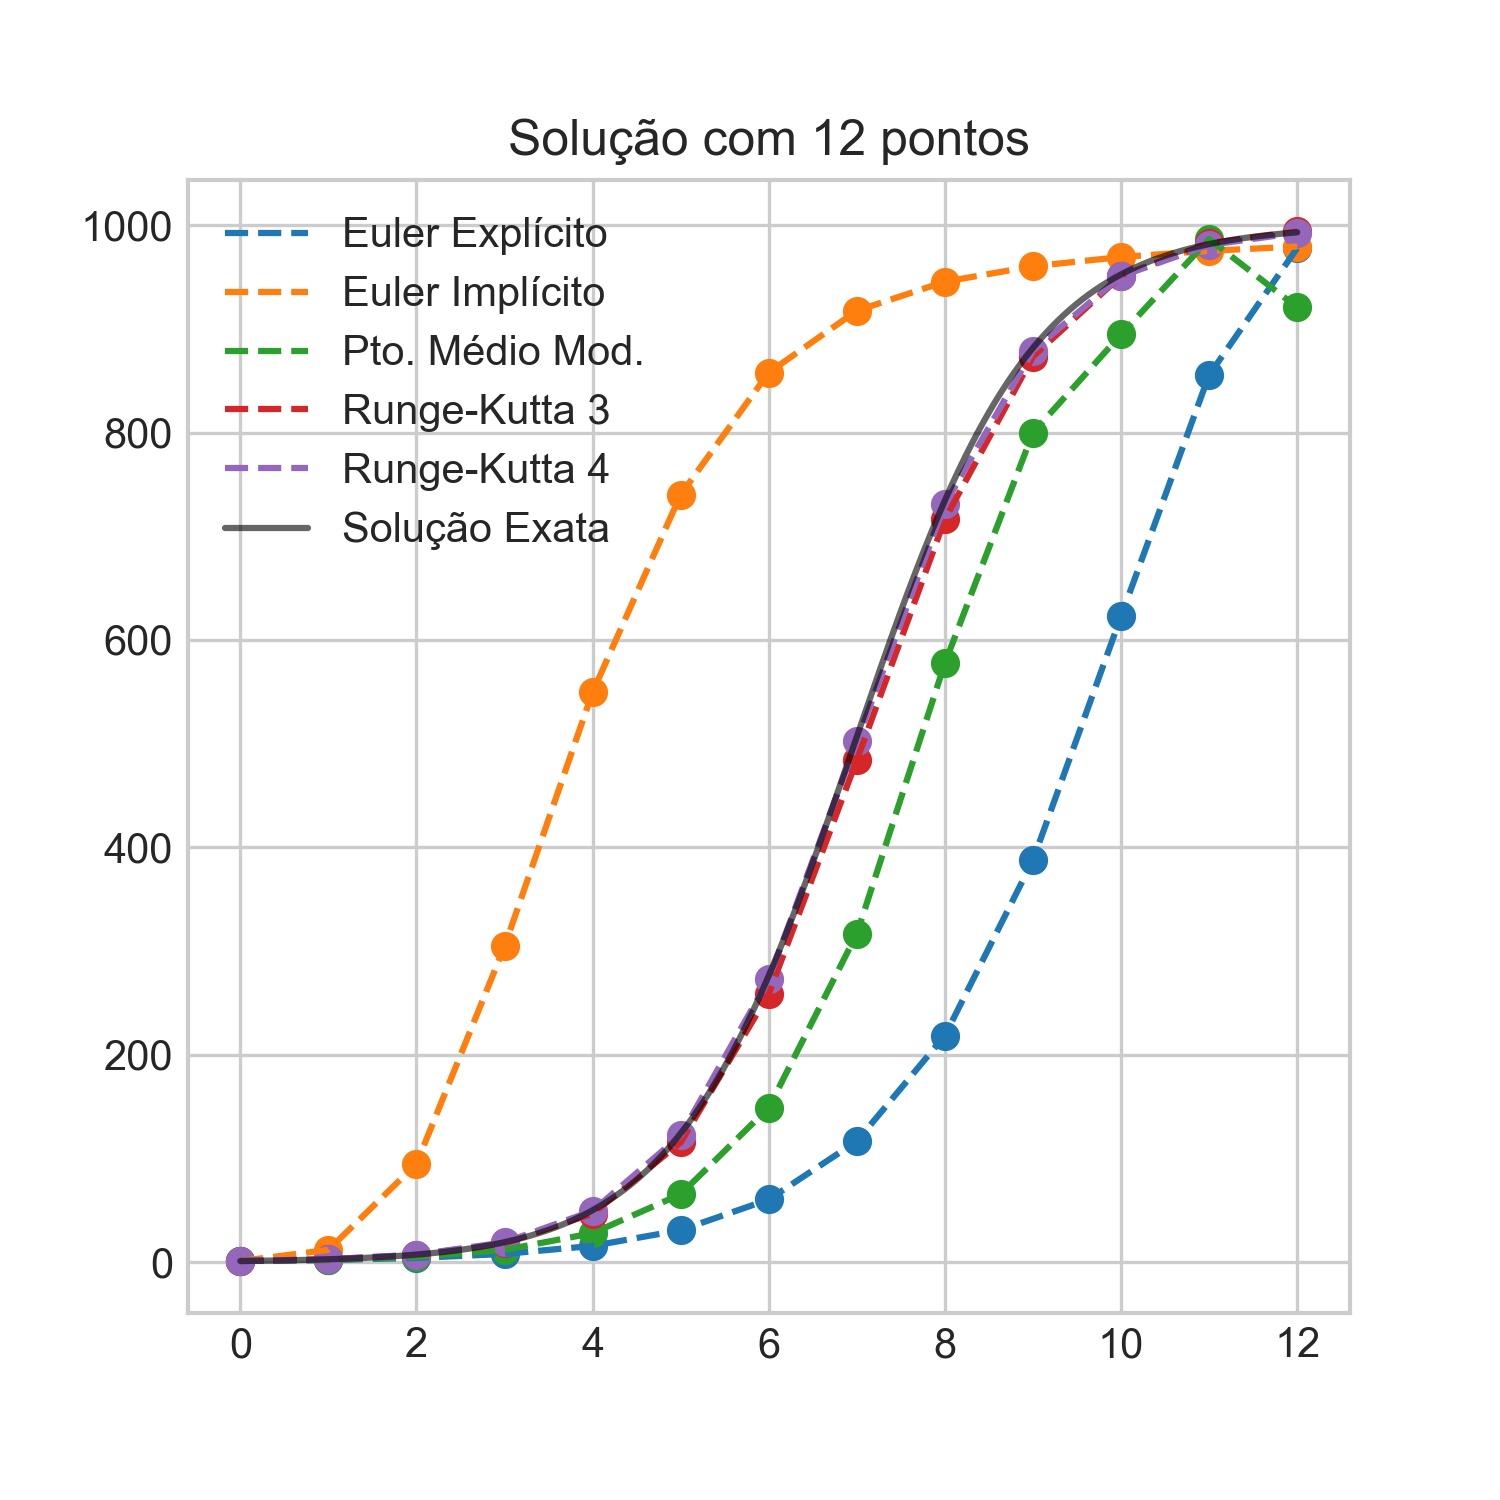
\includegraphics[height=7.8cm, width=7.8cm]{disease/solution_12.png}}
		\subfigure[]{
			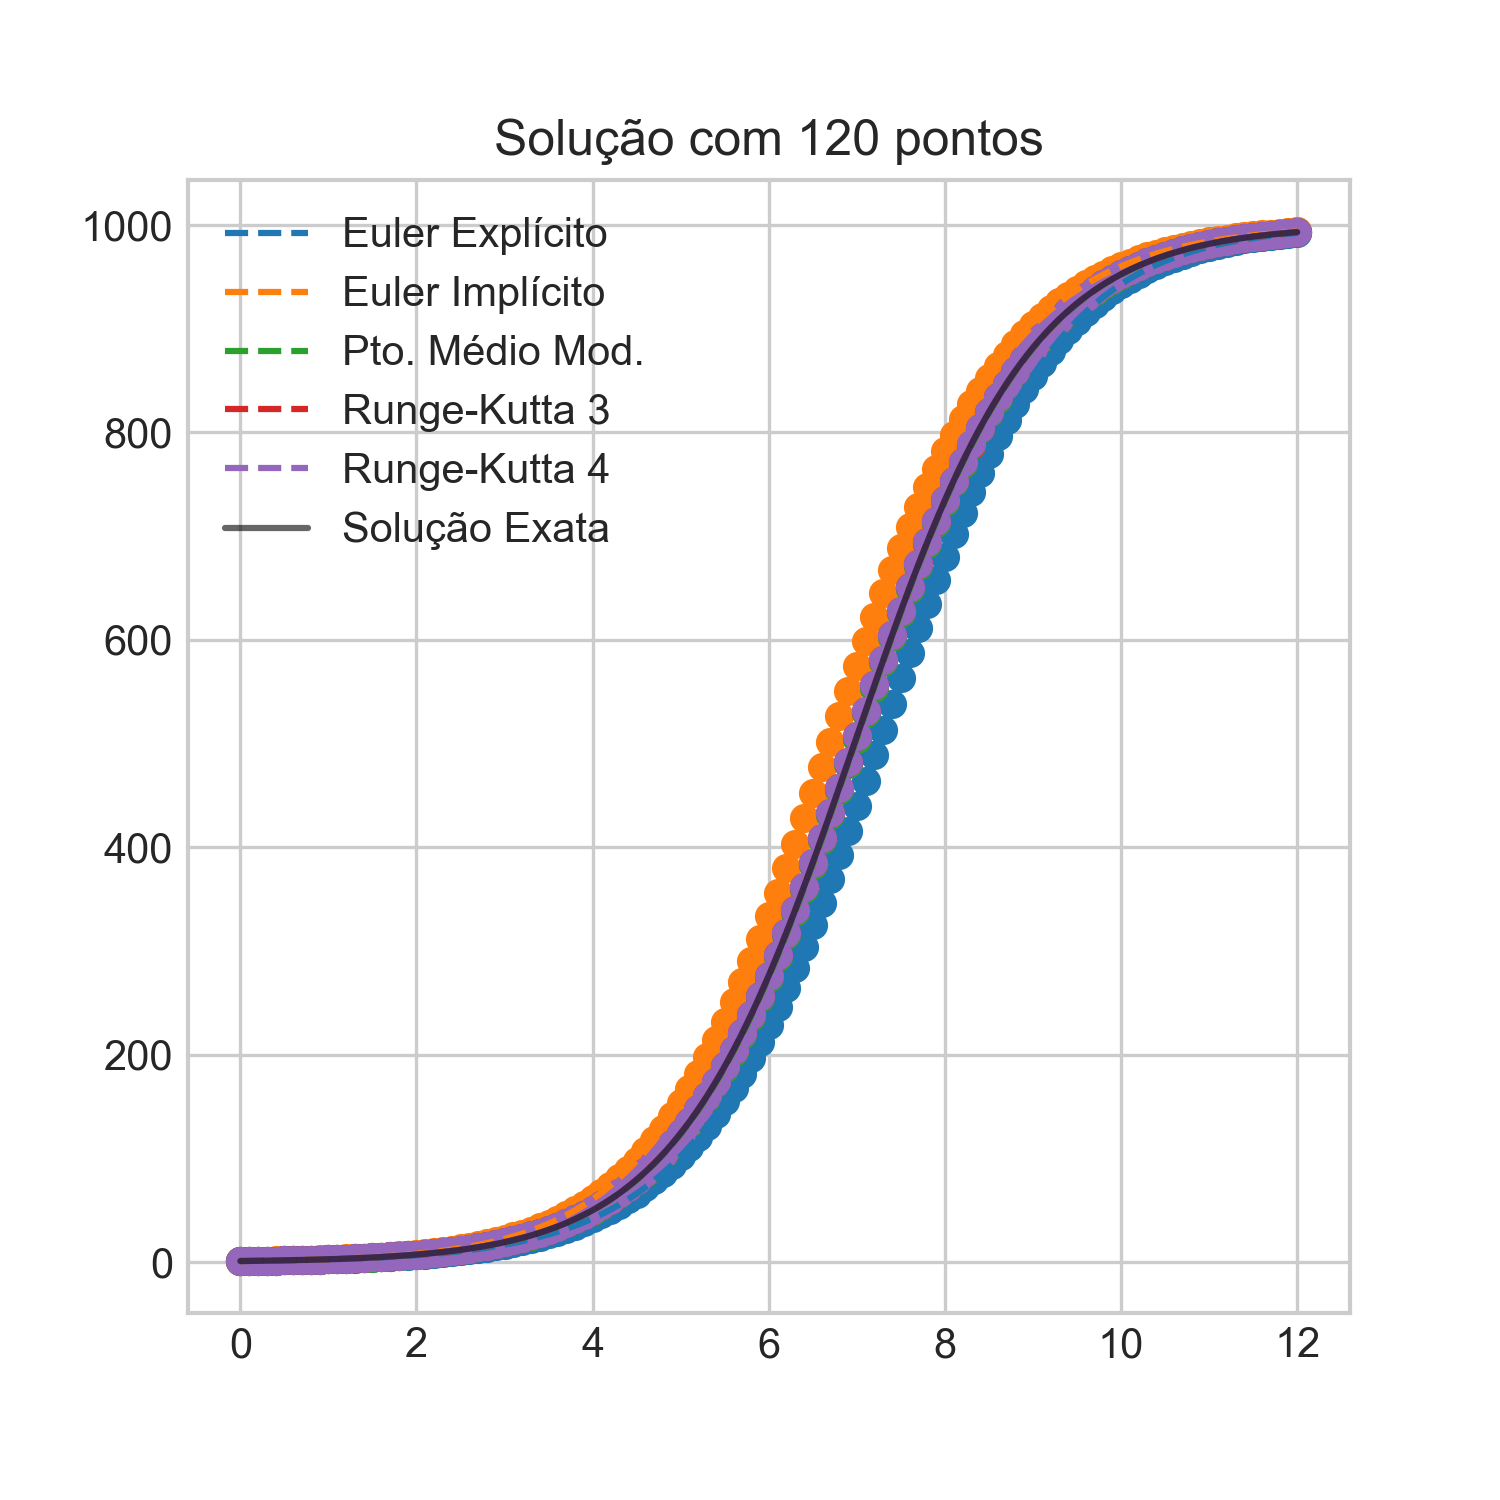
\includegraphics[height=7.8cm, width=7.8cm]{disease/solution_120.png}}
	}
	\mbox{
		\subfigure[]{
			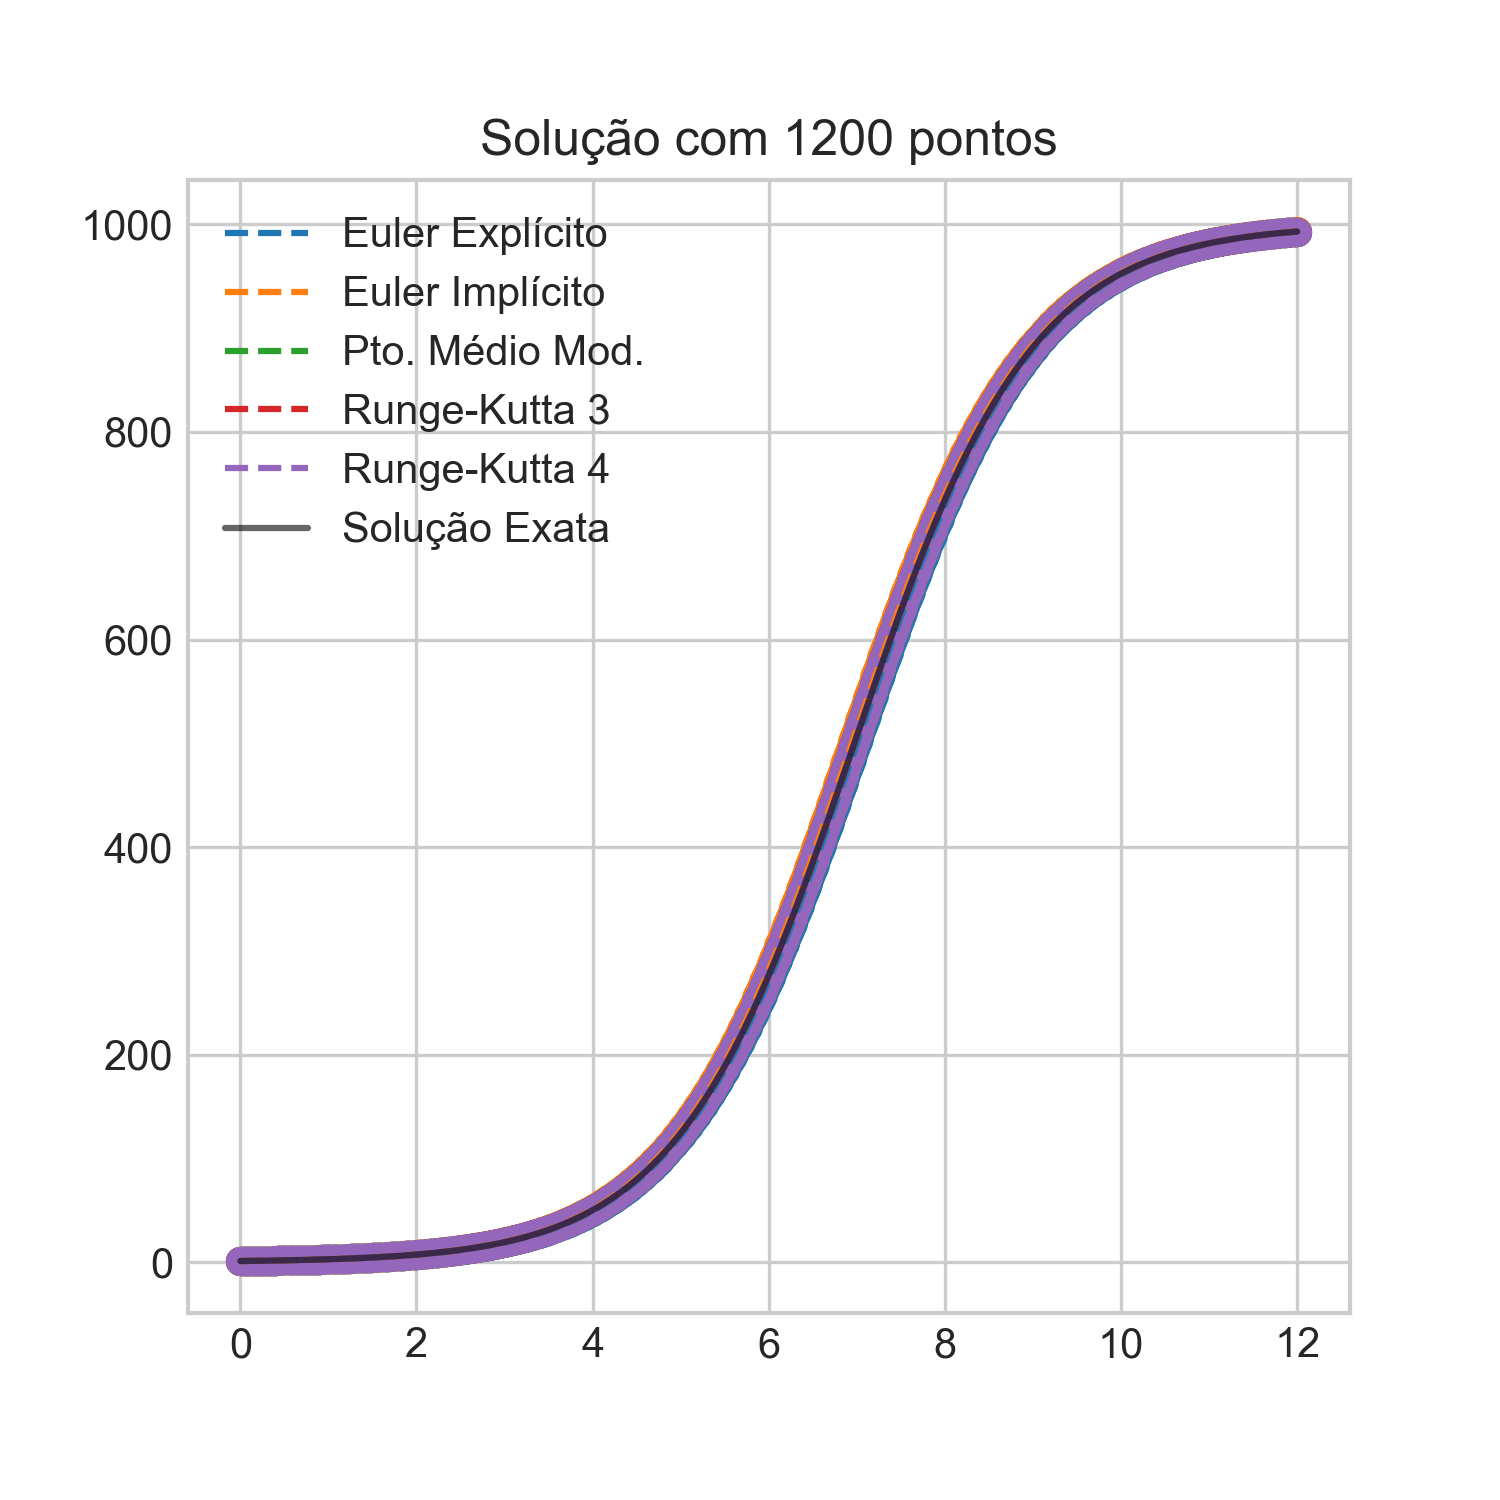
\includegraphics[height=7.8cm, width=7.8cm]{disease/solution_1200.png}}
		\subfigure[]{
			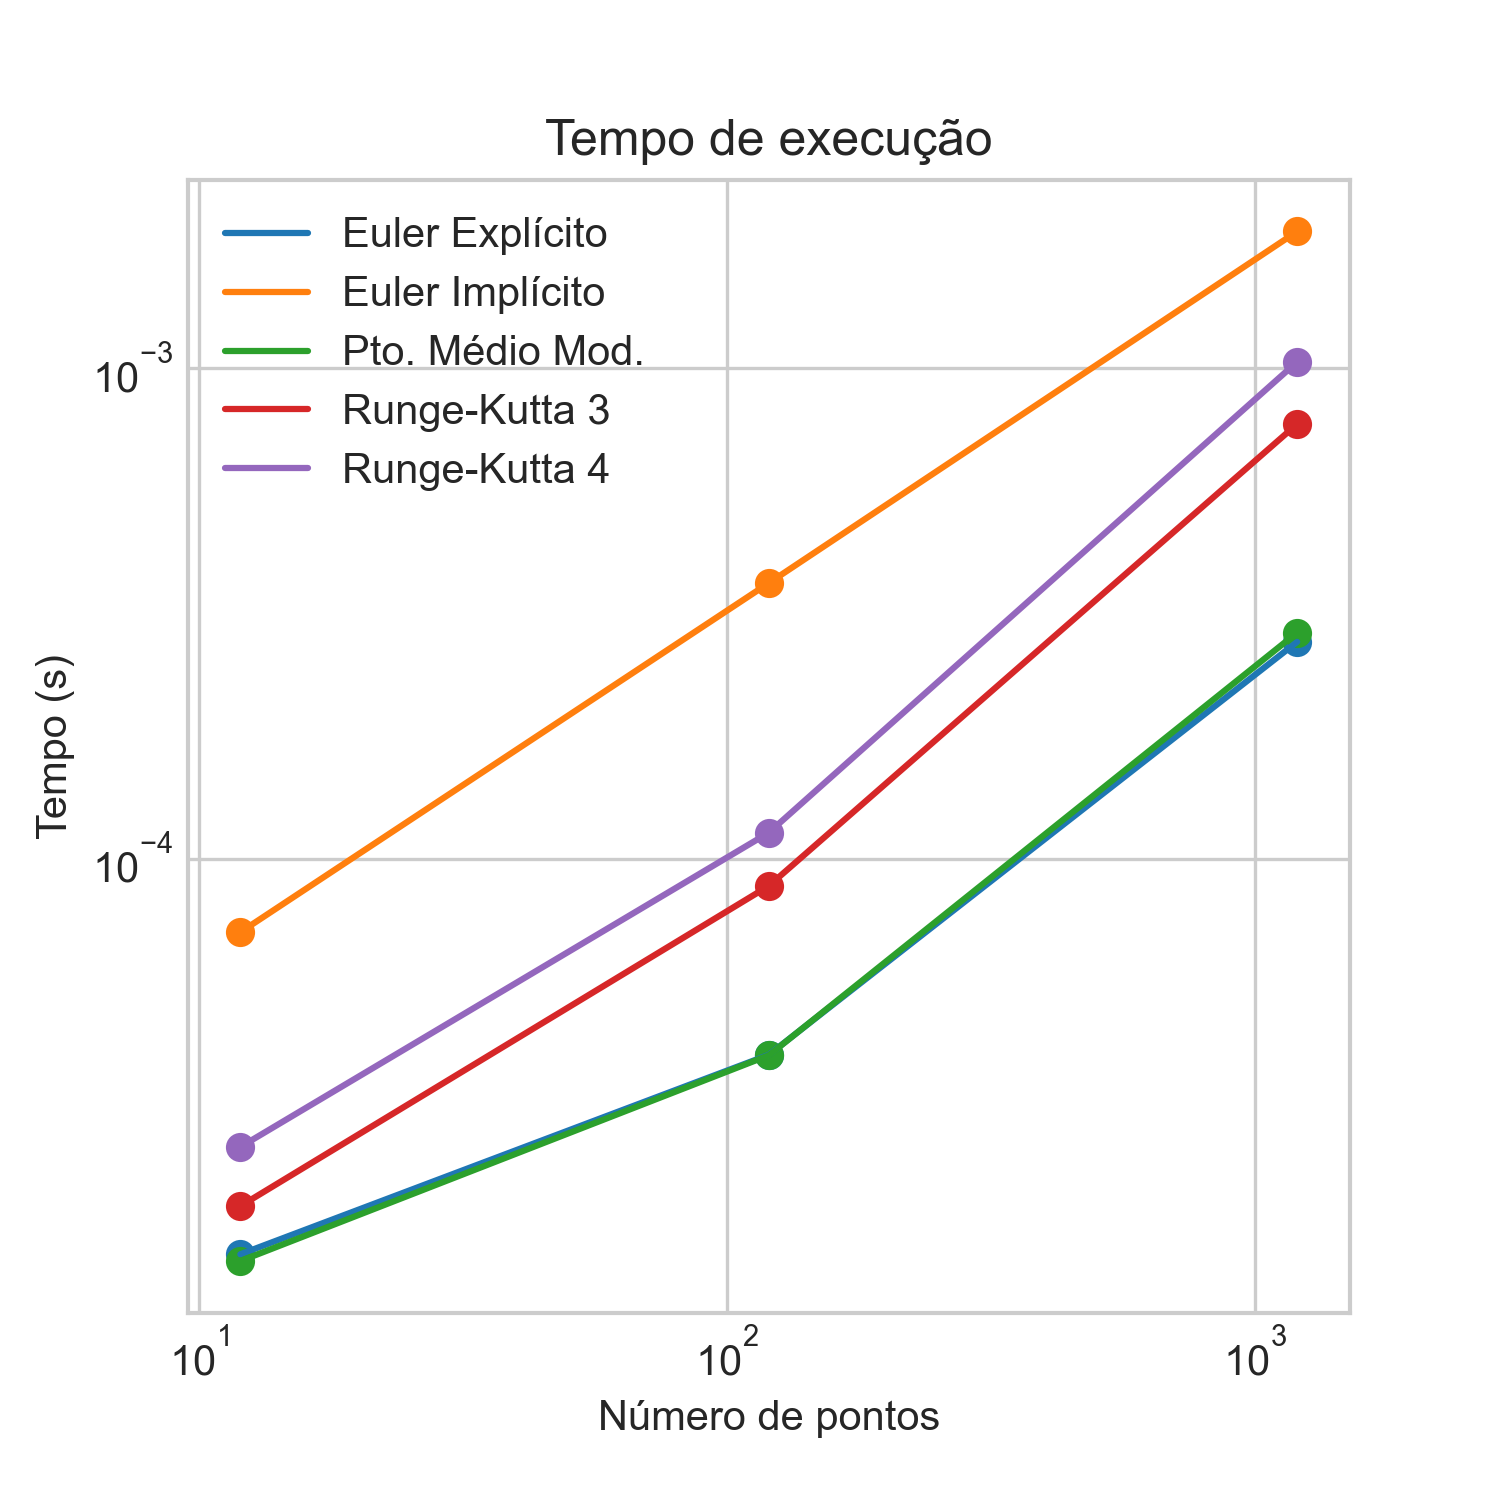
\includegraphics[height=7.8cm, width=7.8cm]{disease/timings.png}}
	}
	\caption{(a) Solução com malha grossa; (b) Solução com malha intermediária; (c) Solução com malha fina; (d) Tempos de execução de cada método. }
    \label{img:ex1_plots}
\end{figure}

Pode-se observar que à medida que o tamanho da malha diminui, as soluções se aproximam cada vez mais da solução analítica, resultando em uma redução do erro de aproximação. Além disso, o tempo de execução aumenta proporcionalmente ao número de pontos da malha.

Outra medida útil para avaliar a precisão dos métodos é o erro relativo, definido como $E_{r} = \Bigg|\dfrac{y_i - y(t_i)}{y(t_i)}\Bigg|$ para $y(t_i) \ne 0$. A Tabela \ref{tab:ex1_relative_errors} apresenta o erro relativo médio para cada método em toda a malha.

% TODO: FIX THIS (2023)
\begin{table}\label{tabela-exemplo1}
	\centering
	\begin{tabular}{|c|c|c|c|c|}
		\hline
		Ordem & \backslashbox{Método}{Pontos} & $12$                   & $120$                  & $1200$                 \\
		\hline
        \rule{0pt}{3ex} 
		1&Euler Explícito & $5.03 \times 10^{-1}$ & $8.50 \times 10^{-2}$ & $9.17 \times 10^{-3}$ \\ \rule{0pt}{3ex} 
        1&Euler Implícito & $4.06 \times 10^{+0}$ & $1.02 \times 10^{-1}$ & $9.34 \times 10^{-3}$ \\ \rule{0pt}{3ex} 
        2&Ponto Médio Modificado & $2.57 \times 10^{-1}$ & $4.08 \times 10^{-3}$ & $4.10 \times 10^{-5}$ \\ \rule{0pt}{3ex} 
        3&Runge-Kutta 3 & $3.22 \times 10^{-2}$ & $6.39 \times 10^{-5}$ & $6.85 \times 10^{-8}$ \\ \rule{0pt}{3ex} 
        4&Runge-Kutta 4 & $6.66 \times 10^{-3}$ & $1.32 \times 10^{-6}$ & $1.42 \times 10^{-10}$ \\
		\hline
		
	\end{tabular}
 \caption{Erros relativos dos métodos computacionais aplicados no PVI do Exemplo $1$.}
 \label{tab:ex1_relative_errors}
\end{table}

Nota-se novamente que métodos de maior ordem tendem a convergir mais rapidamente do que os de menor ordem. Além disso, ao reduzir o espaçamento da malha, diminui-se também o erro relativo médio. Por exemplo, ao diminuir o tamanho da malha em uma magnitude de $10^1$, reduziu-se aproximadamente $10^4$ no erro médio do método de Runge-Kutta de quarta ordem. Na Tabela \ref{tab:ex1_effective_order}, pode-se analisar a ordem efetiva de cada método utilizando (\ref{effective_order}).

\begin{table}[H]
    \centering
    \begin{tabular}{|c|c|}
        \hline
        Método & Ordem de acurácia efetiva\\
        \hline \rule{0pt}{2.5ex} 
         Euler Explícito & $1.01812$\\\rule{0pt}{2.5ex} 
         Euler Implícito & $0.98333$\\\rule{0pt}{2.5ex} 
         Ponto Médio Modificado & $2.00104$\\\rule{0pt}{2.5ex} 
         Runge-Kutta 3 & $2.87502$\\\rule{0pt}{2.5ex} 
         Runge-Kutta 4 & $3.99328$\\
         \hline
    \end{tabular}
    \caption{Ordem efetiva dos erros para cada método estudado.}
    \label{tab:ex1_effective_order}
\end{table}



\subsection{Segundo problema: capacidade de carga}\label{problem-2} \quad
O segundo problema são os estudos de Lotka-Volterra sobre a Lei de Crescimento de Populações, que exploram a capacidade de carga de um meio utilizando funções logísticas. O objetivo é determinar o tamanho máximo da população de uma espécie dada a capacidade máxima do ambiente em que vive e outros fatores, como a taxa de crescimento natural e o número atual de indivíduos vivos. Busca-se assim, simular a evolução do número de indivíduos vivos na população utilizando os métodos iterativos.


O problema pode ser descrito matematicamente com:
\begin{equation}\label{carry_equation_to_be_solved}
	\frac{dP}{dt} = \beta \cdot P \cdot \bigg(1 - \frac{P}{K}\bigg)
\end{equation}

onde:\begin{itemize}
\item $P$ é o número de indivíduos vivos; 
\item $\beta$ é a taxa de crescimento da população;
\item $K$ é a capacidade de carga máxima do sistema;
\item $t$ é a variável de tempo, medida em anos;
\end{itemize}

As equações logísticas são conhecidas pela sua forma em S. Seja $P_0$ a população inicial do problema (\ref{carry_equation_to_be_solved}), observa-se que no início do intervalo a população crescerá lentamente, pois há poucos indivíduos para reproduzirem. A partir desse ponto, $P$ crescerá cada vez mais rapidamente até se aproximar do valor de K, momento em que o crescimento diminuirá, uma vez que $\lim_{P\to K} \big(1 - \frac{P}{K}\big) = 0$. A solução geral de um problema de Lei de Crescimento de Populações de Lotka-Volterra é descrita como:
\begin{equation*}
 P(t) = \dfrac{K}{\dfrac{K - P_0}{P_0} \cdot e^{-\beta t} + 1}
\end{equation*}

Para $\beta = 1$, $K = 1000$, $P_0 = 100$ e o intervalo $[0, 12]$, o PVI a ser resolvido é dado por:
\begin{equation}\label{pvi_carrying-capacity}
    \begin{cases}
	\dfrac{dP}{dt} = \cdot P \cdot \bigg(1 - \dfrac{P}{1000}\bigg) & \\
        P(0) = 100 & t \in [0, 12]
    \end{cases}
\end{equation}
Para este problema, a solução analítica é apresentada como:
\begin{equation*}
    P(t) = \dfrac{3000}{\dfrac{3000 - 100}{100} \cdot e^{-t} + 1} = \dfrac{3000}{29e^{-t} + 1}
\end{equation*}
Utilizando os métodos estudados, a solução numérica obitida para o problema (\ref{pvi_carrying-capacity}) é ilustrada na Figura \ref{img:carry_plots}.
\begin{figure}[H]
	\centering
	\mbox{
		\subfigure[]{
			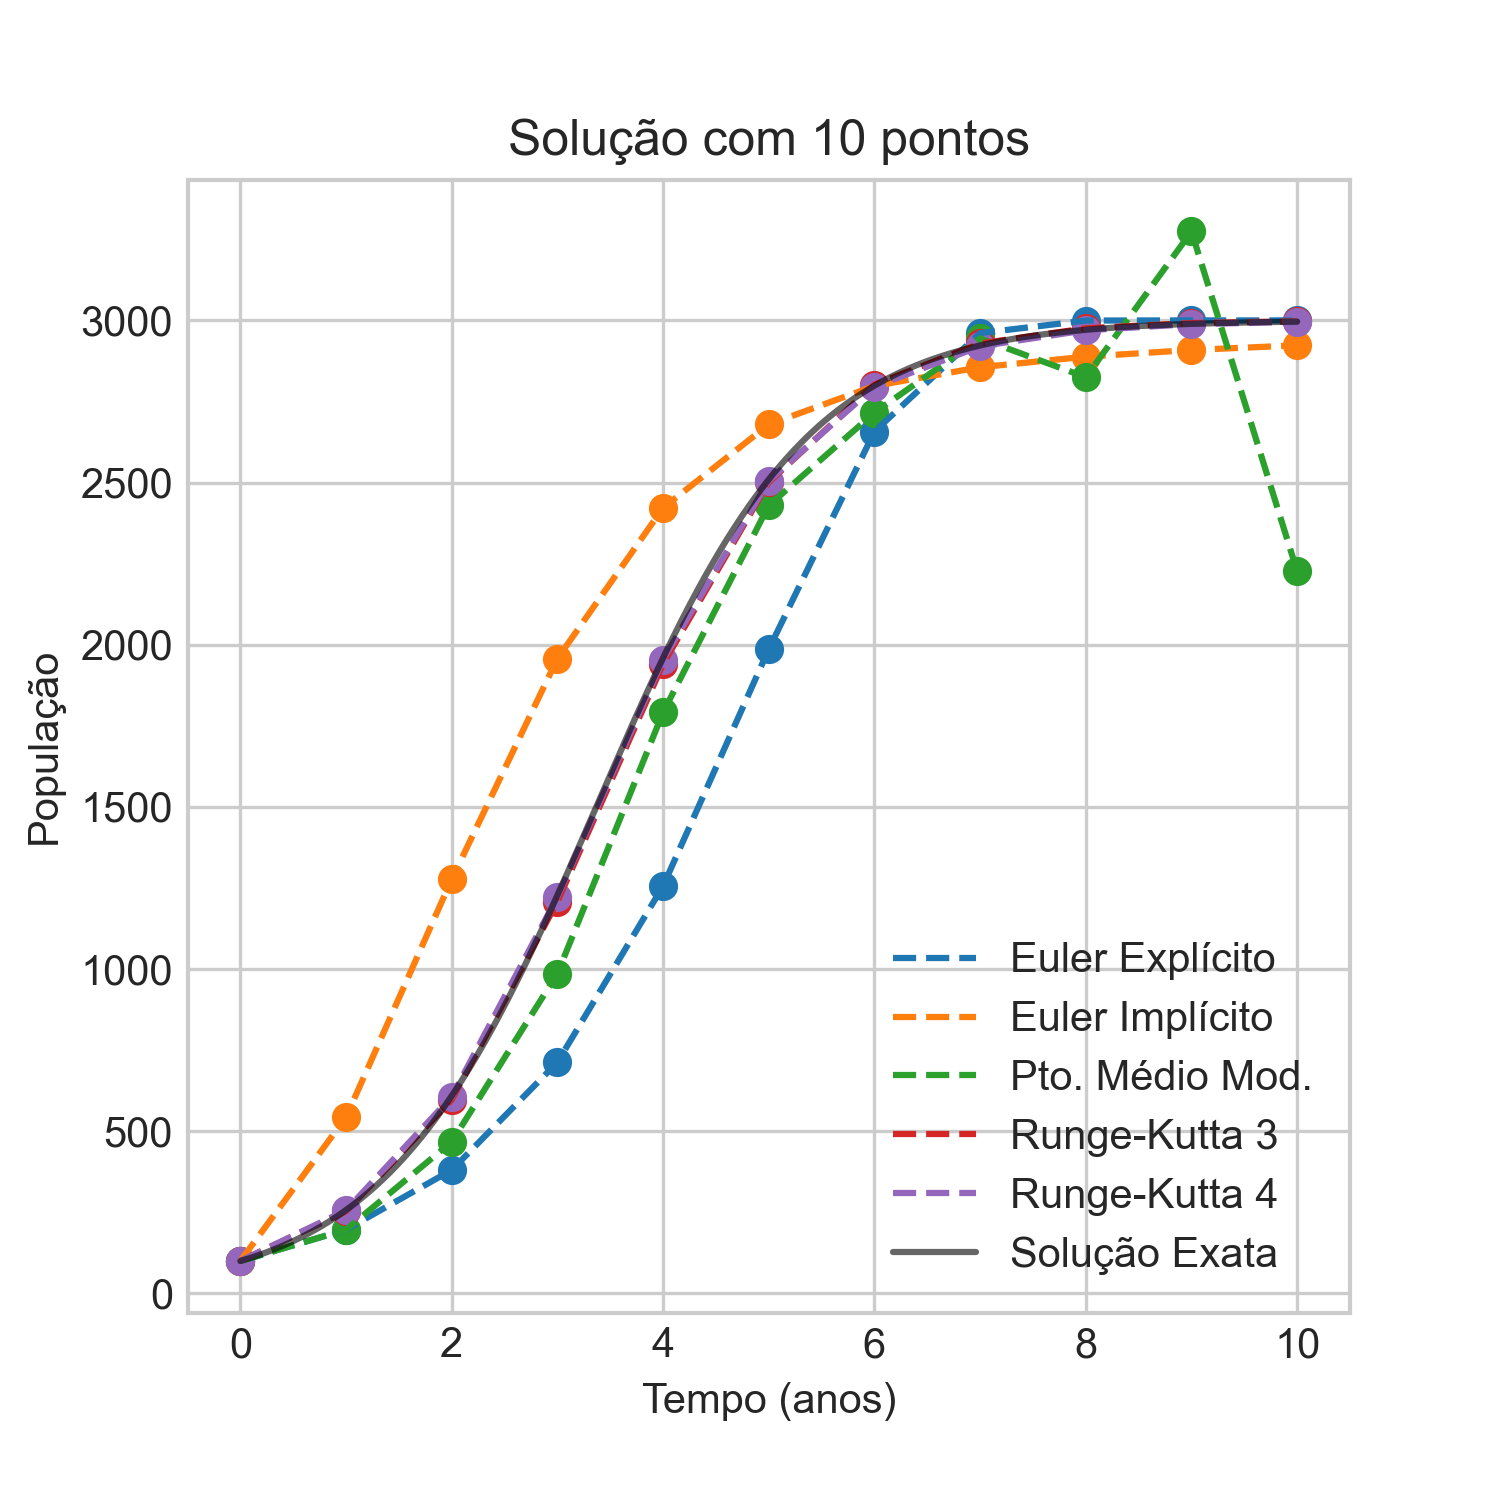
\includegraphics[height=7.8cm, width=7.8cm]{carry-capacity/carry-solution_10_300dpi.png}}
		\subfigure[]{
			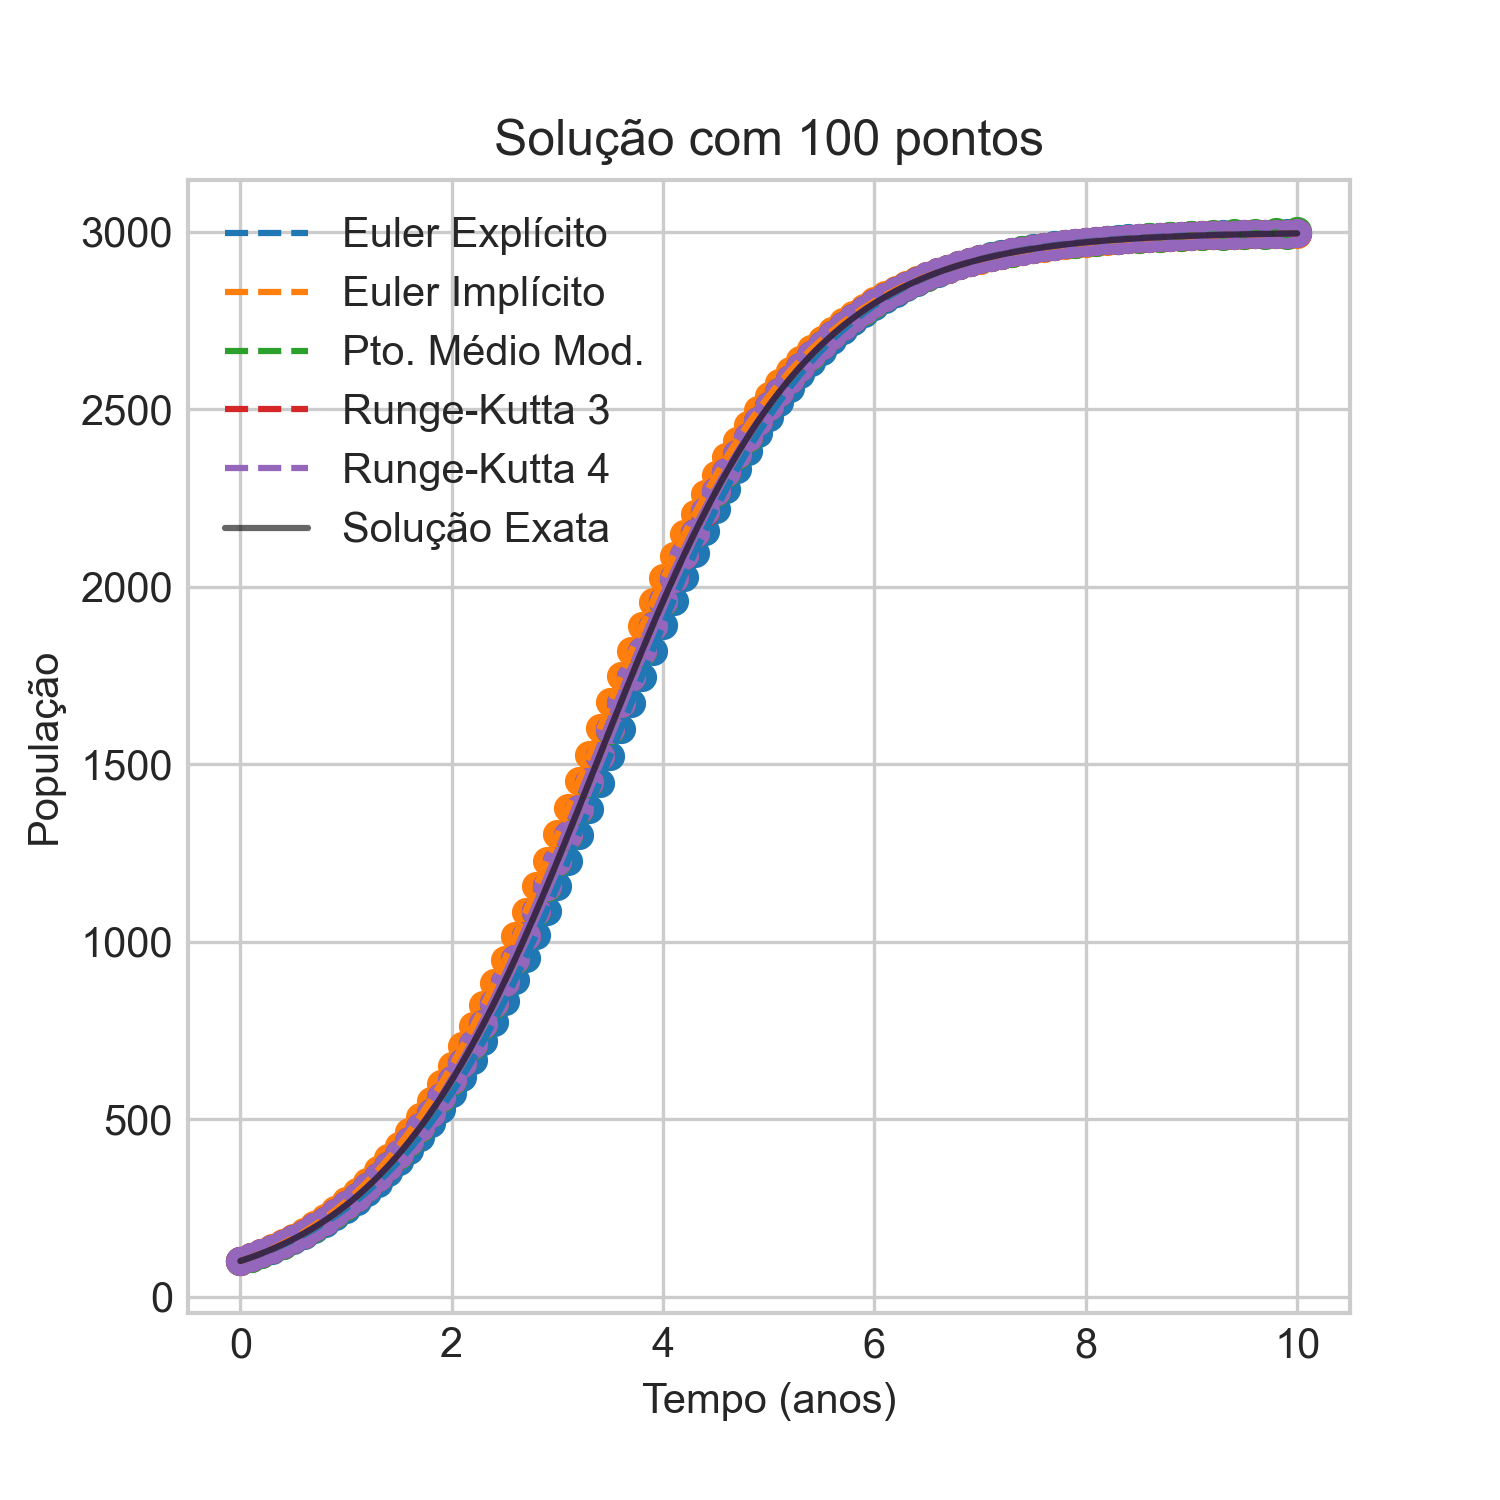
\includegraphics[height=7.8cm, width=7.8cm]{carry-capacity/carry-solution_100_300dpi.png}}
	}
	\mbox{
		\subfigure[]{
			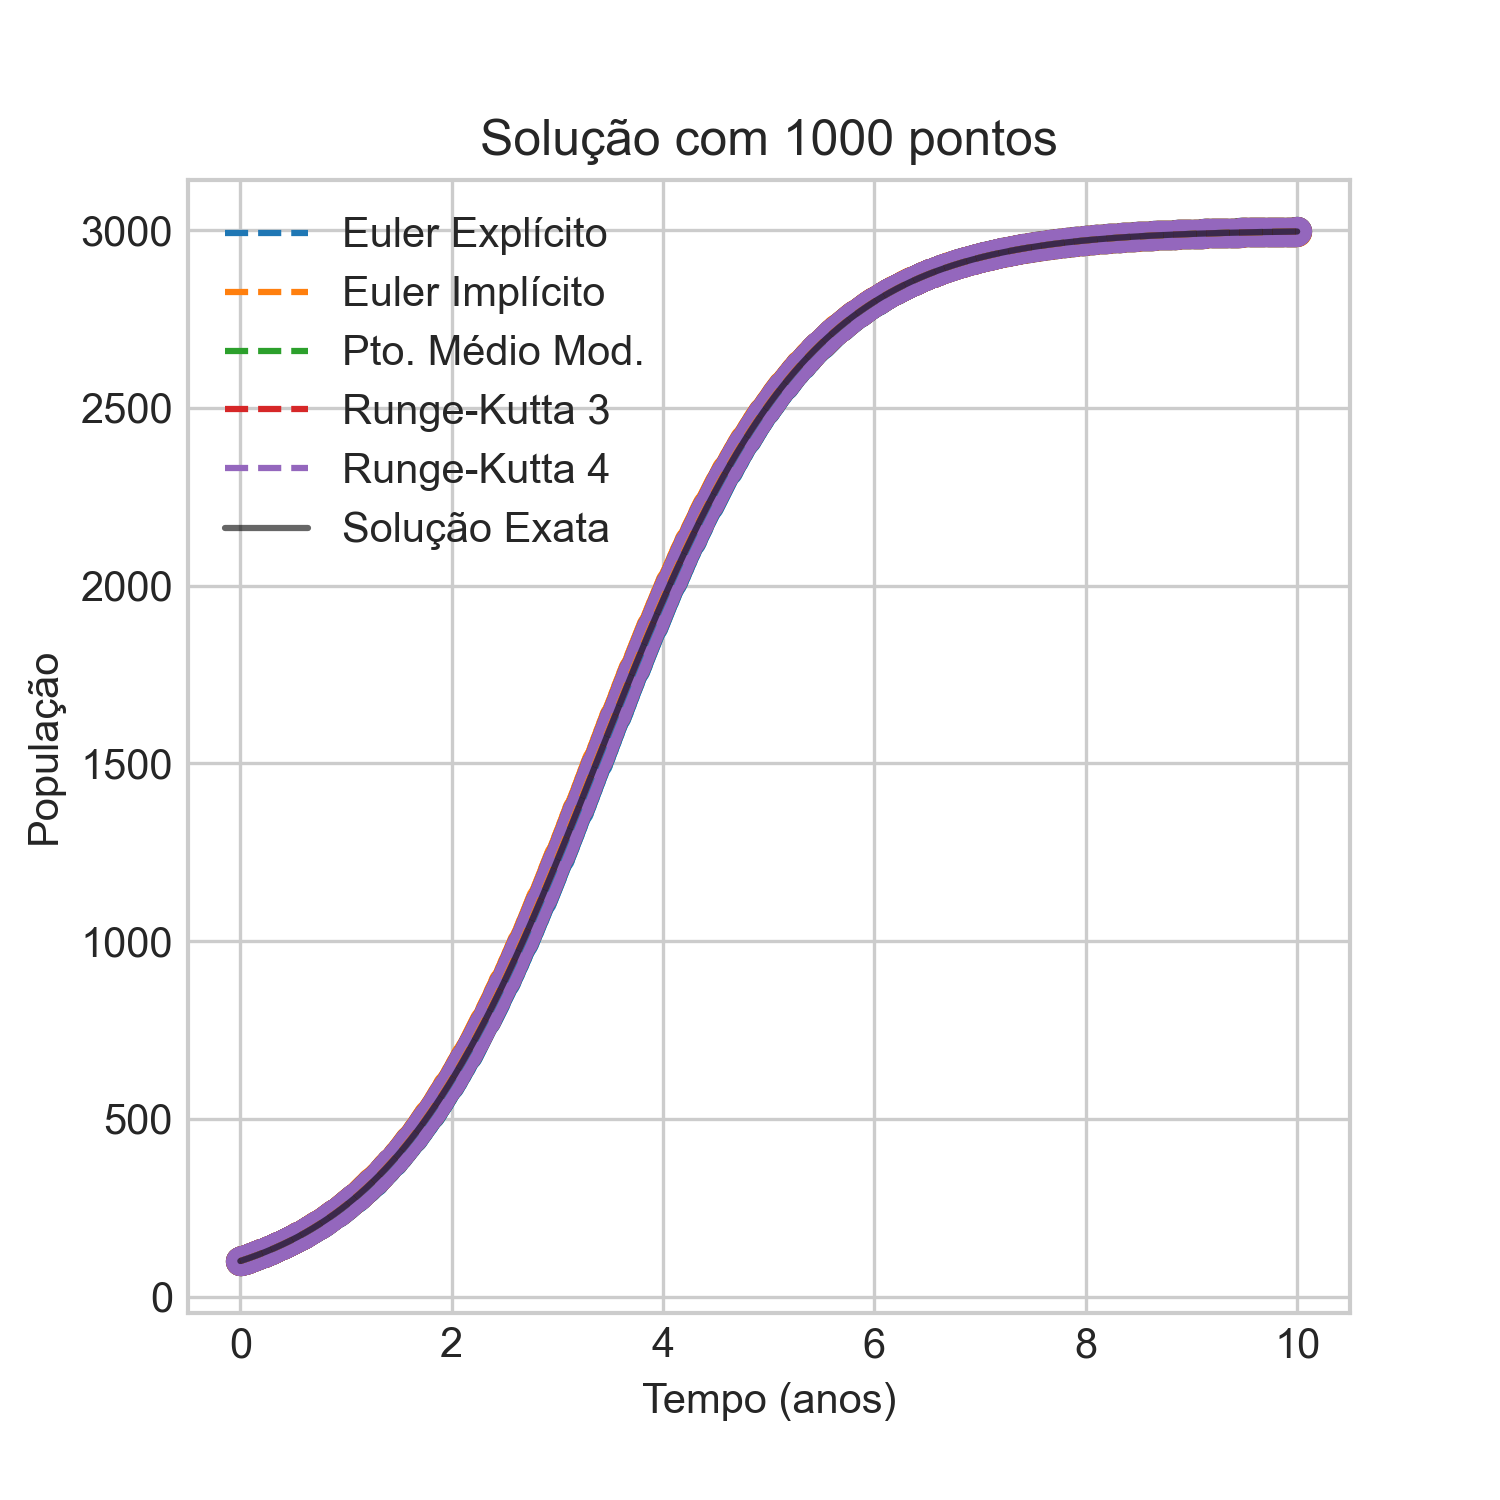
\includegraphics[height=7.8cm, width=7.8cm]{carry-capacity/carry-solution_1000_300dpi.png}}
		\subfigure[]{
			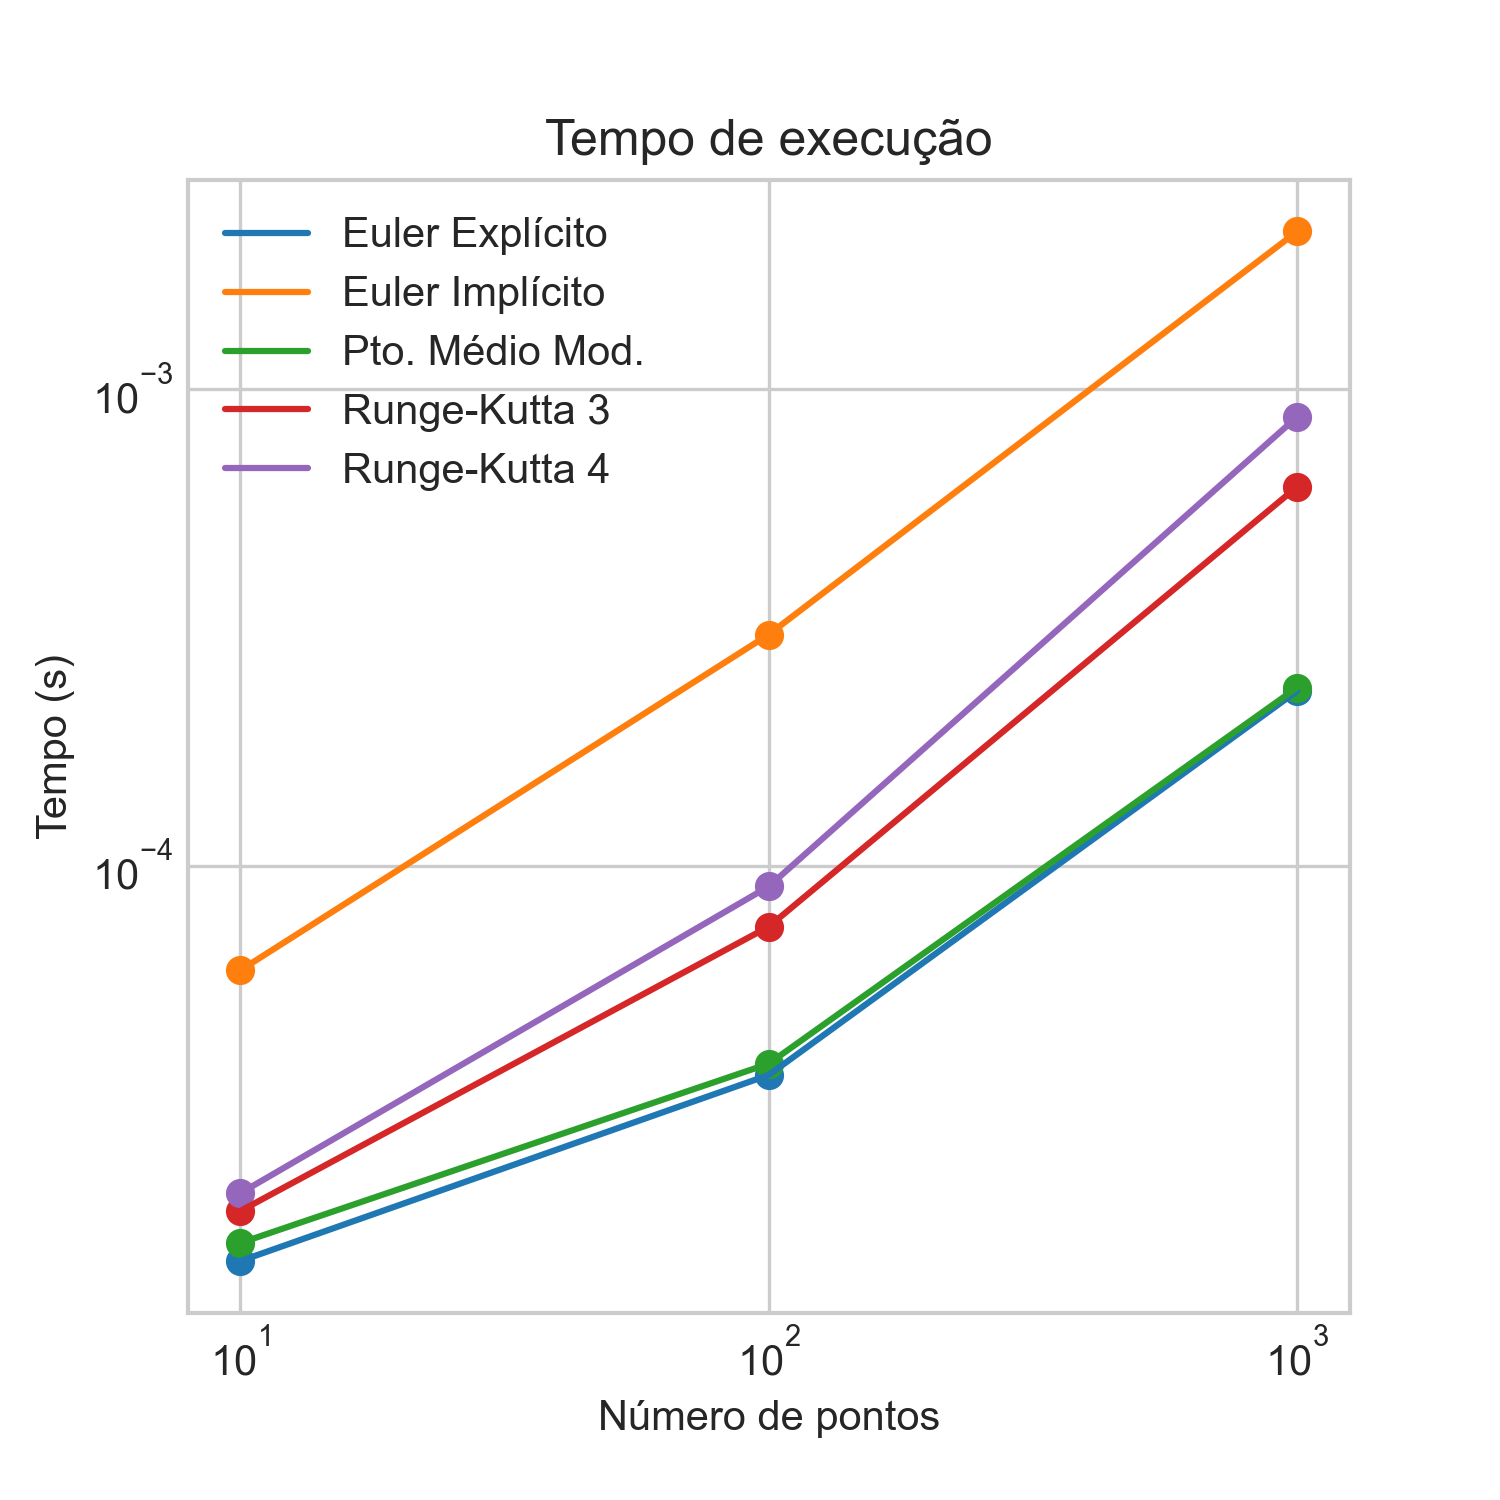
\includegraphics[height=7.8cm, width=7.8cm]{carry-capacity/timings-300dpi.png}}
	}
	\caption{(a) Solução com malha grossa; (b) Solução com malha intermediária; (c) Solução com malha fina; (d) Tempos de execução de cada método. }
    \label{img:carry_plots}
\end{figure}

Assim como no primeiro problema, ao reduzir o tamanho da malha, as soluções convergem para a solução analítica. O erro relativo médio, para cada método, está descrito na Tabela \ref{tab:carry_relative_errors}.

% TODO: Fix this (2023)
\begin{table}\label{tabela-carry}
	\centering
	\begin{tabular}{|c|c|c|c|c|}
		\hline
		Ordem & \backslashbox{Método}{Pontos} & $10$                   & $100$                  & $1000$                 \\
		\hline
        \rule{0pt}{3ex} 
		1&Euler Explícito & $1.67 \times 10^{-1}$ & $2.11 \times 10^{-2}$ & $2.17 \times 10^{-3}$ \\ \rule{0pt}{3ex}
        1&Euler Implícito & $3.19 \times 10^{-1}$ & $2.25 \times 10^{-2}$ & $2.18 \times 10^{-3}$ \\ \rule{0pt}{3ex}
        2&Ponto Médio Modificado & $9.64 \times 10^{-2}$ & $1.30 \times 10^{-3}$ & $1.31 \times 10^{-5}$ \\ \rule{0pt}{3ex}
        3&Runge-Kutta 3 & $6.65 \times 10^{-3}$ & $1.14 \times 10^{-5}$ & $1.21 \times 10^{-8}$ \\ \rule{0pt}{3ex}
        4&Runge-Kutta 4 & $1.76 \times 10^{-3}$ & $2.89 \times 10^{-7}$ & $3.05 \times 10^{-11}$ \\
		\hline
		
	\end{tabular}
 \caption{Erros relativos dos métodos computacionais aplicados no PVI do Exemplo $1$.}
 \label{tab:carry_relative_errors}
\end{table}

Observa-se novamente que os métodos de maior ordem tendem a convergir mais rapidamente do que os métodos de menor ordem. Além disso, ao diminuir o espaçamento da malha, foi possível reduzir o erro relativo médio: por exemplo, ao reduzir o tamanho da malha em uma ordem de magnitude ($10^1$), obteve-se uma redução no erro médio de cada método na ordem de $10^{O(h)}$. Vale ressaltar que a ordem efetiva de cada método pode ser analisada na Tabela \ref{tab:carry_effective_order}, utilizando a equação (\ref{effective_order}).

\begin{table}[H]
    \centering
    \begin{tabular}{|c|c|}
        \hline
        Método & Ordem de acurácia efetiva\\
        \hline \rule{0pt}{2.5ex} 
        Euler Explícito & 0.99593\\\rule{0pt}{2.5ex} 
        Euler Implícito & 1.00228\\\rule{0pt}{2.5ex} 
        Ponto Médio Modificado & 1.99196\\\rule{0pt}{2.5ex} 
        Runge-Kutta 3 & 3.04741\\\rule{0pt}{2.5ex} 
        Runge-Kutta 4 & 4.01748\\
         \hline
    \end{tabular}
    \caption{Ordem efetiva dos erros para cada método estudado.}
    \label{tab:carry_effective_order}
\end{table}

Por fim, embora a estabilidade dos métodos utilizados não tenha sido abordada neste trabalho, vale ressaltar que em ambos os exemplos o método do Ponto Médio Modificado (uma adaptação das diferenças centradas) apresentou instabilidade em sua solução, sendo mais evidente em malhas mais grossas. Embora o método do Ponto Médio Modificado seja de ordem superior ao método de Euler Explícito, mantendo um custo computacional semelhante, como pode ser visto nas Figuras $\ref{img:ex1_plots}d$ e $\ref{img:carry_plots}d$, está mais sujeito a instabilidade numérica e requer condições mais restritas de espaçamento de malha \cite{ascher2008numerical}.

%%%%%%%%%%%%%%%%%%%%%%%%%%%%%%%%%%%%%%%%%%%%%%%%
\subsection{Terceiro problema: populações de predadores e presas}\label{problem-3} \quad
O terceiro problema consiste em uma equação competitiva de Lotka-Volterra \cite{goel1971} que modela a dinâmica de populações de predadores e presas. Esse modelo considera duas populações, uma de predadores $A$ e outra de presas $B$, tal que:

\emph{
	No início de um período, as presas se reproduzem e, ao final do período, cada indivíduo em média produz $r$ filhos. As presas não morrem naturalmente, mas estão sujeitas a serem predadas com uma probabilidade $p$. Por outro lado, os predadores morrem rapidamente de fome e, se não são alimentados, morrem na proporção $s$. A taxa de reprodução dos predadores está relacionada à sua capacidade de alimentação, que depende da quantidade de presas vivas.}". Adaptado de \cite{burkardt2009}.

O problema em questão é descrito matematicamente por um sistema de equações diferenciais ordinárias, dado por:

\begin{equation*}\label{predator_formula}
	\dfrac{dA}{dt} = r_AAB - sA
\end{equation*}

\begin{equation*}\label{prey_formula}
	\dfrac{dB}{dt} = r_BB - pAB
\end{equation*}

onde:

\begin{itemize}
\item $A$ é o número de predadores vivos;
\item $B$ é o número de presas vivas;
\item $r_A$ é a taxa de crescimento da população de predadores;
\item $r_B$ é a taxa de crescimento da população de presas;
\item $p$ é a probabilidade de uma presa ser capturada e morta por um predador;
\item $s$ é a proporção de predadores que morrem de fome;
\item $t$ é a variável temporal, medida em anos.
\end{itemize}

Considerando as populações iniciais $A_0 = 100$ e $B_0 = 4000$, e os valores dos parâmetros $r_A = 3 \times 10^{-3}$, $r_B = 3$, $p = 1 \times 10^{-2}$ e $s = 10$, obtêm-se o seguinte problema de valor inicial (PVI):

\begin{equation}\label{pvi-predator-prey}
	\begin{cases}
		\dfrac{dA}{dt} = 0.003AB - 10A &                            \\[3mm]
        \dfrac{dB}{dt} = 3B - 0.01AB   &                            \\[2mm]
		A(0) = 100                    &                            \\
        B(0) = 4000                   & \text{ com } t \in [0, 10] 
	\end{cases}
\end{equation}

Para resolver este problema, foram aplicados os métodos de Euler Implícito e Runge-Kutta de 4ª ordem com 500 pontos, visto que ambos geram resultados representativos. Os gráficos das soluções obtidas por estes métodos estão representados nas Figuras \ref{img:explicit_euler_plots} e \ref{img:rk4_plots}.
\begin{figure}[H]
	\centering
	\mbox{
		\subfigure[]{
			\includegraphics[height=8cm, width=8cm]{predator-prey/predator_prey-300dpi-Euler_Implícito-500points-2d.png}}
		\subfigure[]{
			\includegraphics[height=8cm, width=8cm]{predator-prey/predator_prey-300dpi-Euler_Implícito-500points-2d-up.png}}
	}
	\mbox{
		\subfigure[]{
			\includegraphics[height=12cm, width=12cm]{predator-prey/predator_prey-300dpi-Euler_Implícito-500 points.png}}
	}
	\caption{Método de Euler Implícito - (a) Evolução de ambas populações temporalmente; (b) Número de indivíduos vivos simultaneamente em diferentes instantes de tempo; (c) Representação tridimensional da evolução do problema.}
    \label{img:explicit_euler_plots}
\end{figure}

\begin{figure}[H]
	\centering
	\mbox{
		\subfigure[]{
			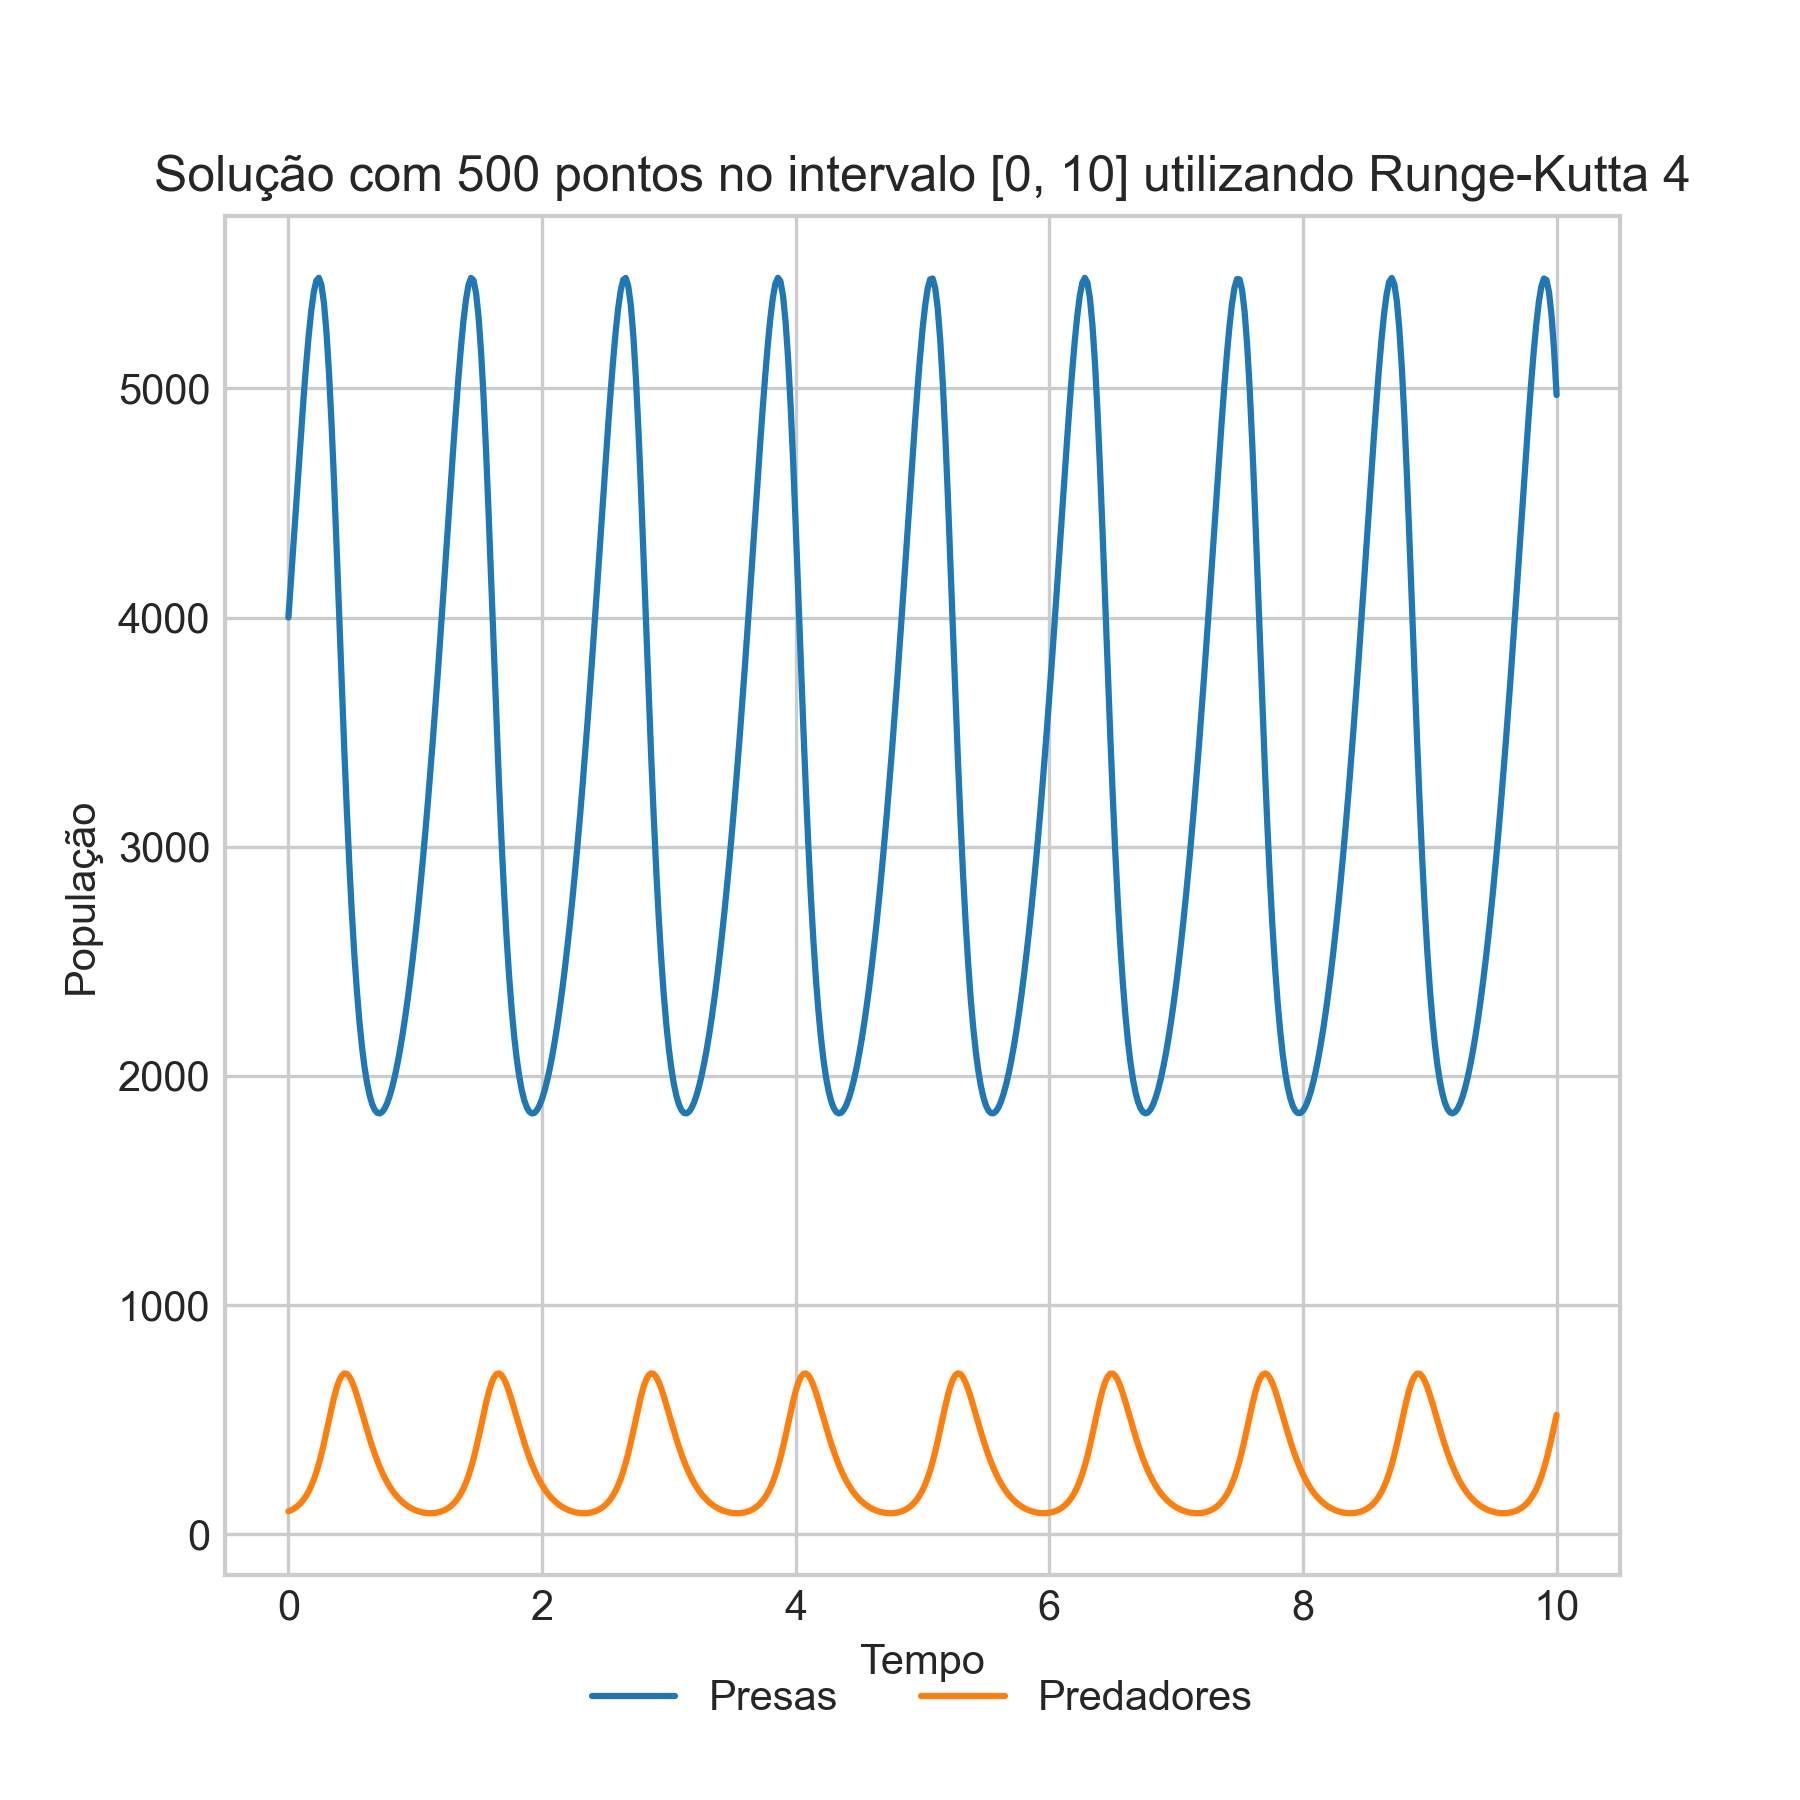
\includegraphics[height=8cm, width=8cm]{predator-prey/predator_prey-300dpi-Runge-Kutta_4-500points-2d.png}}
		\subfigure[]{
			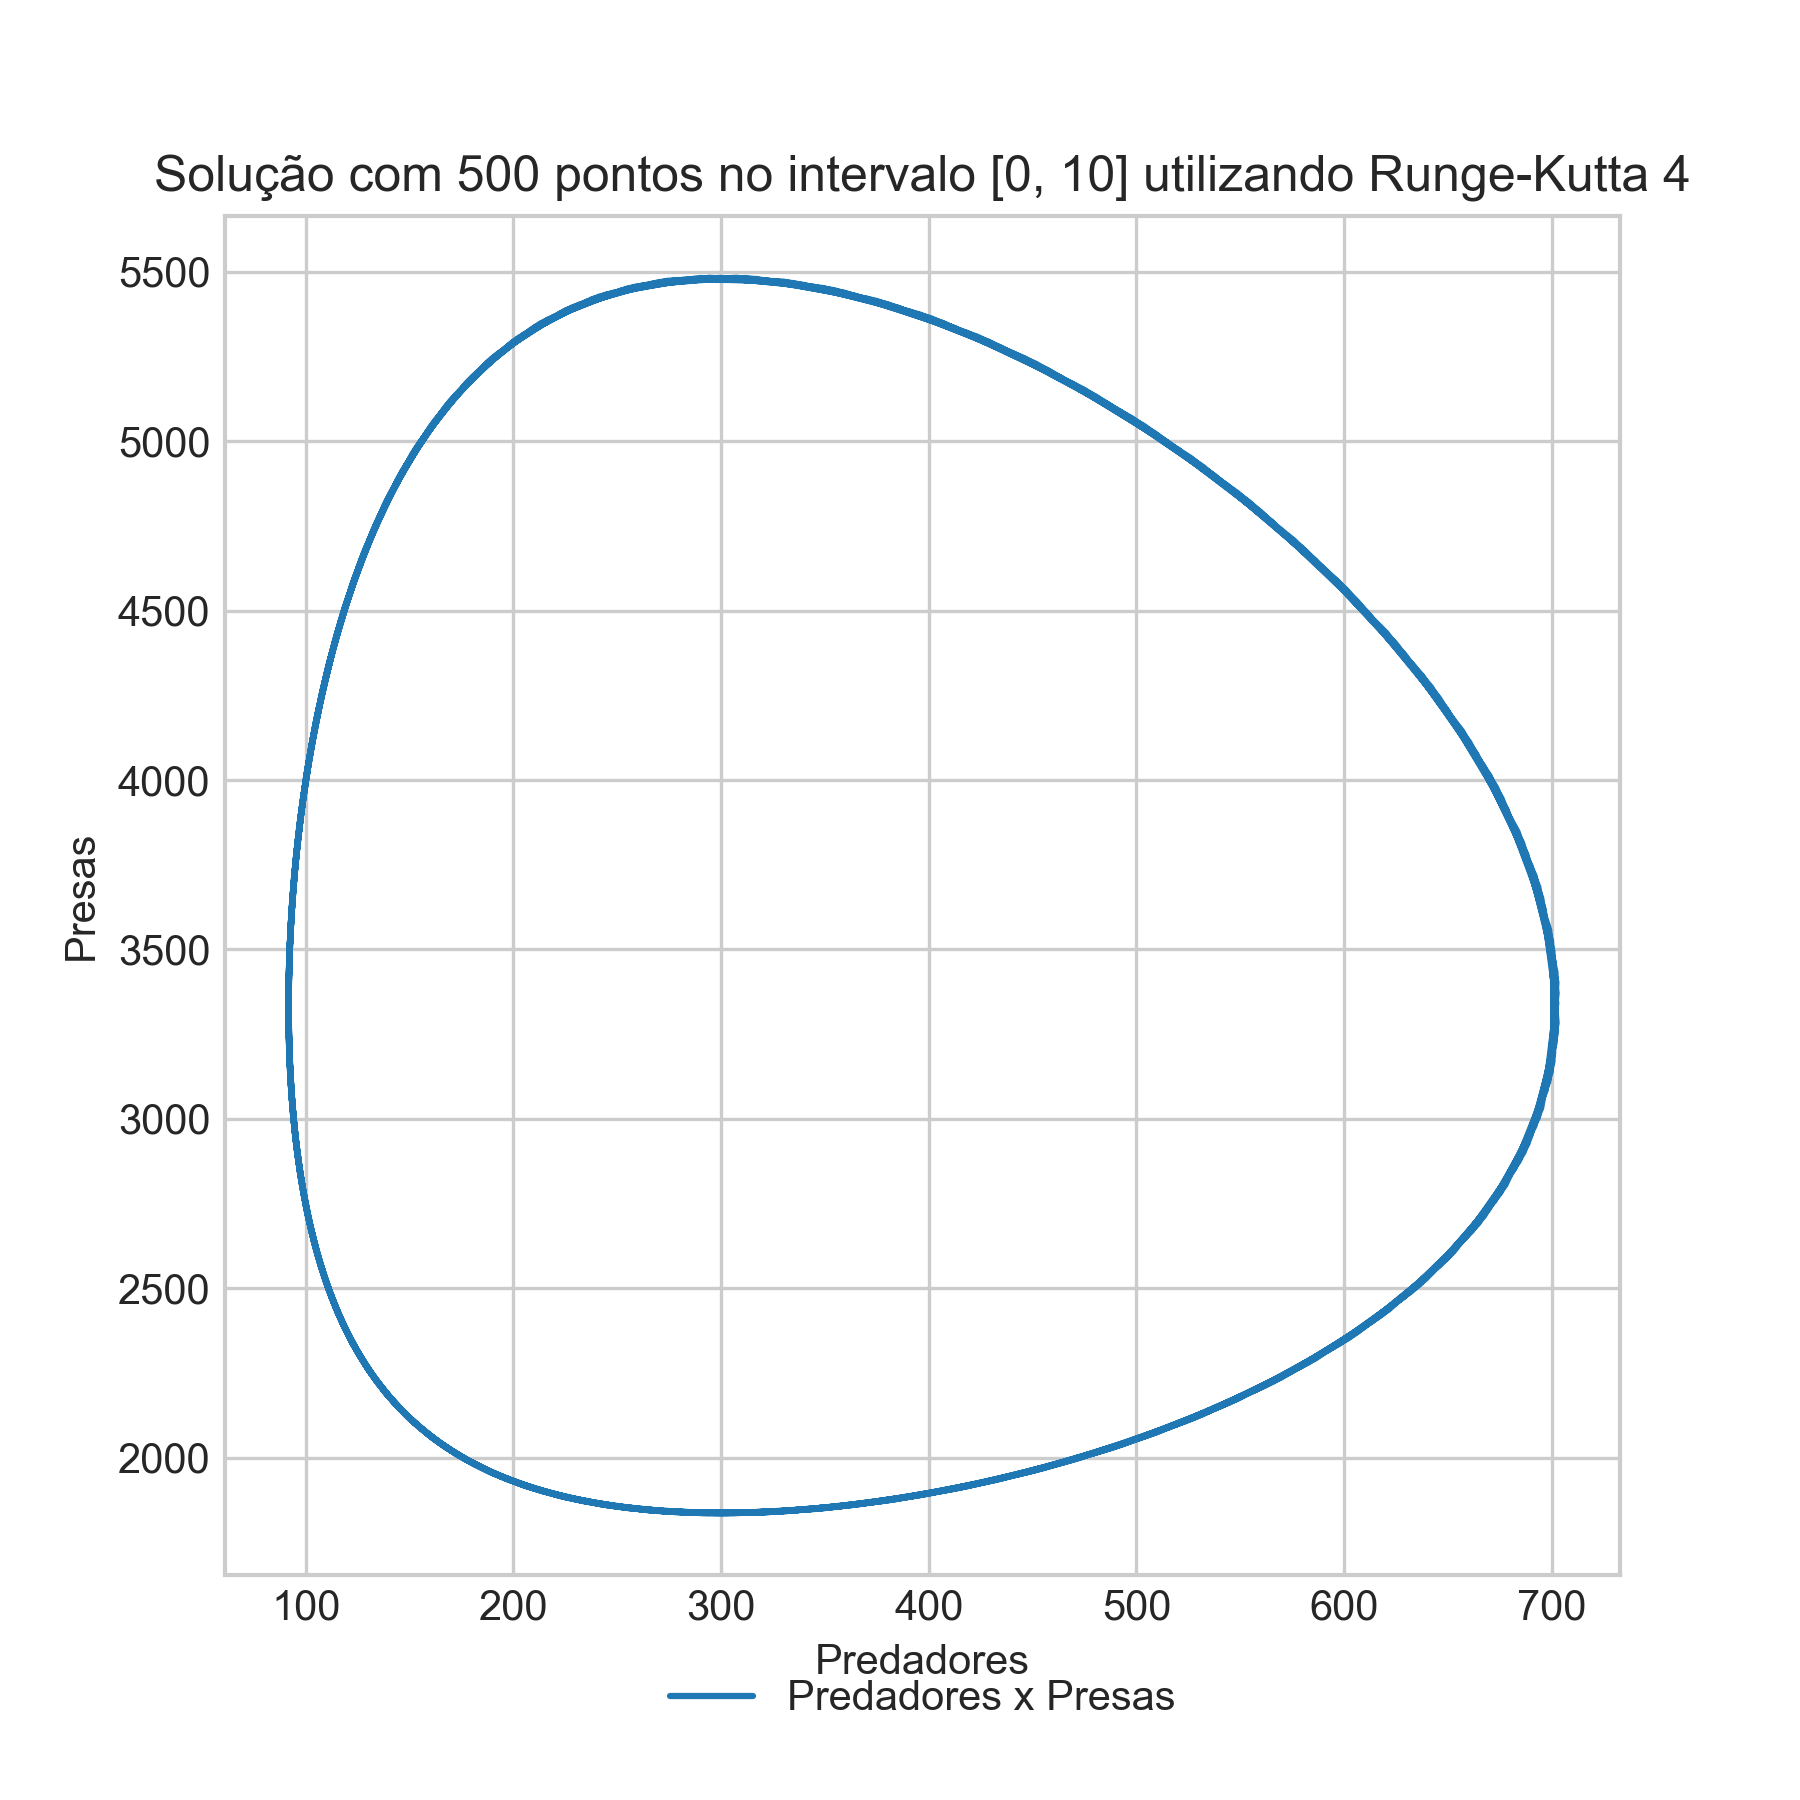
\includegraphics[height=8cm, width=8cm]{predator-prey/predator_prey-300dpi-Runge-Kutta_4-500points-2d-up.png}}
	}
	\mbox{
		\subfigure[]{
			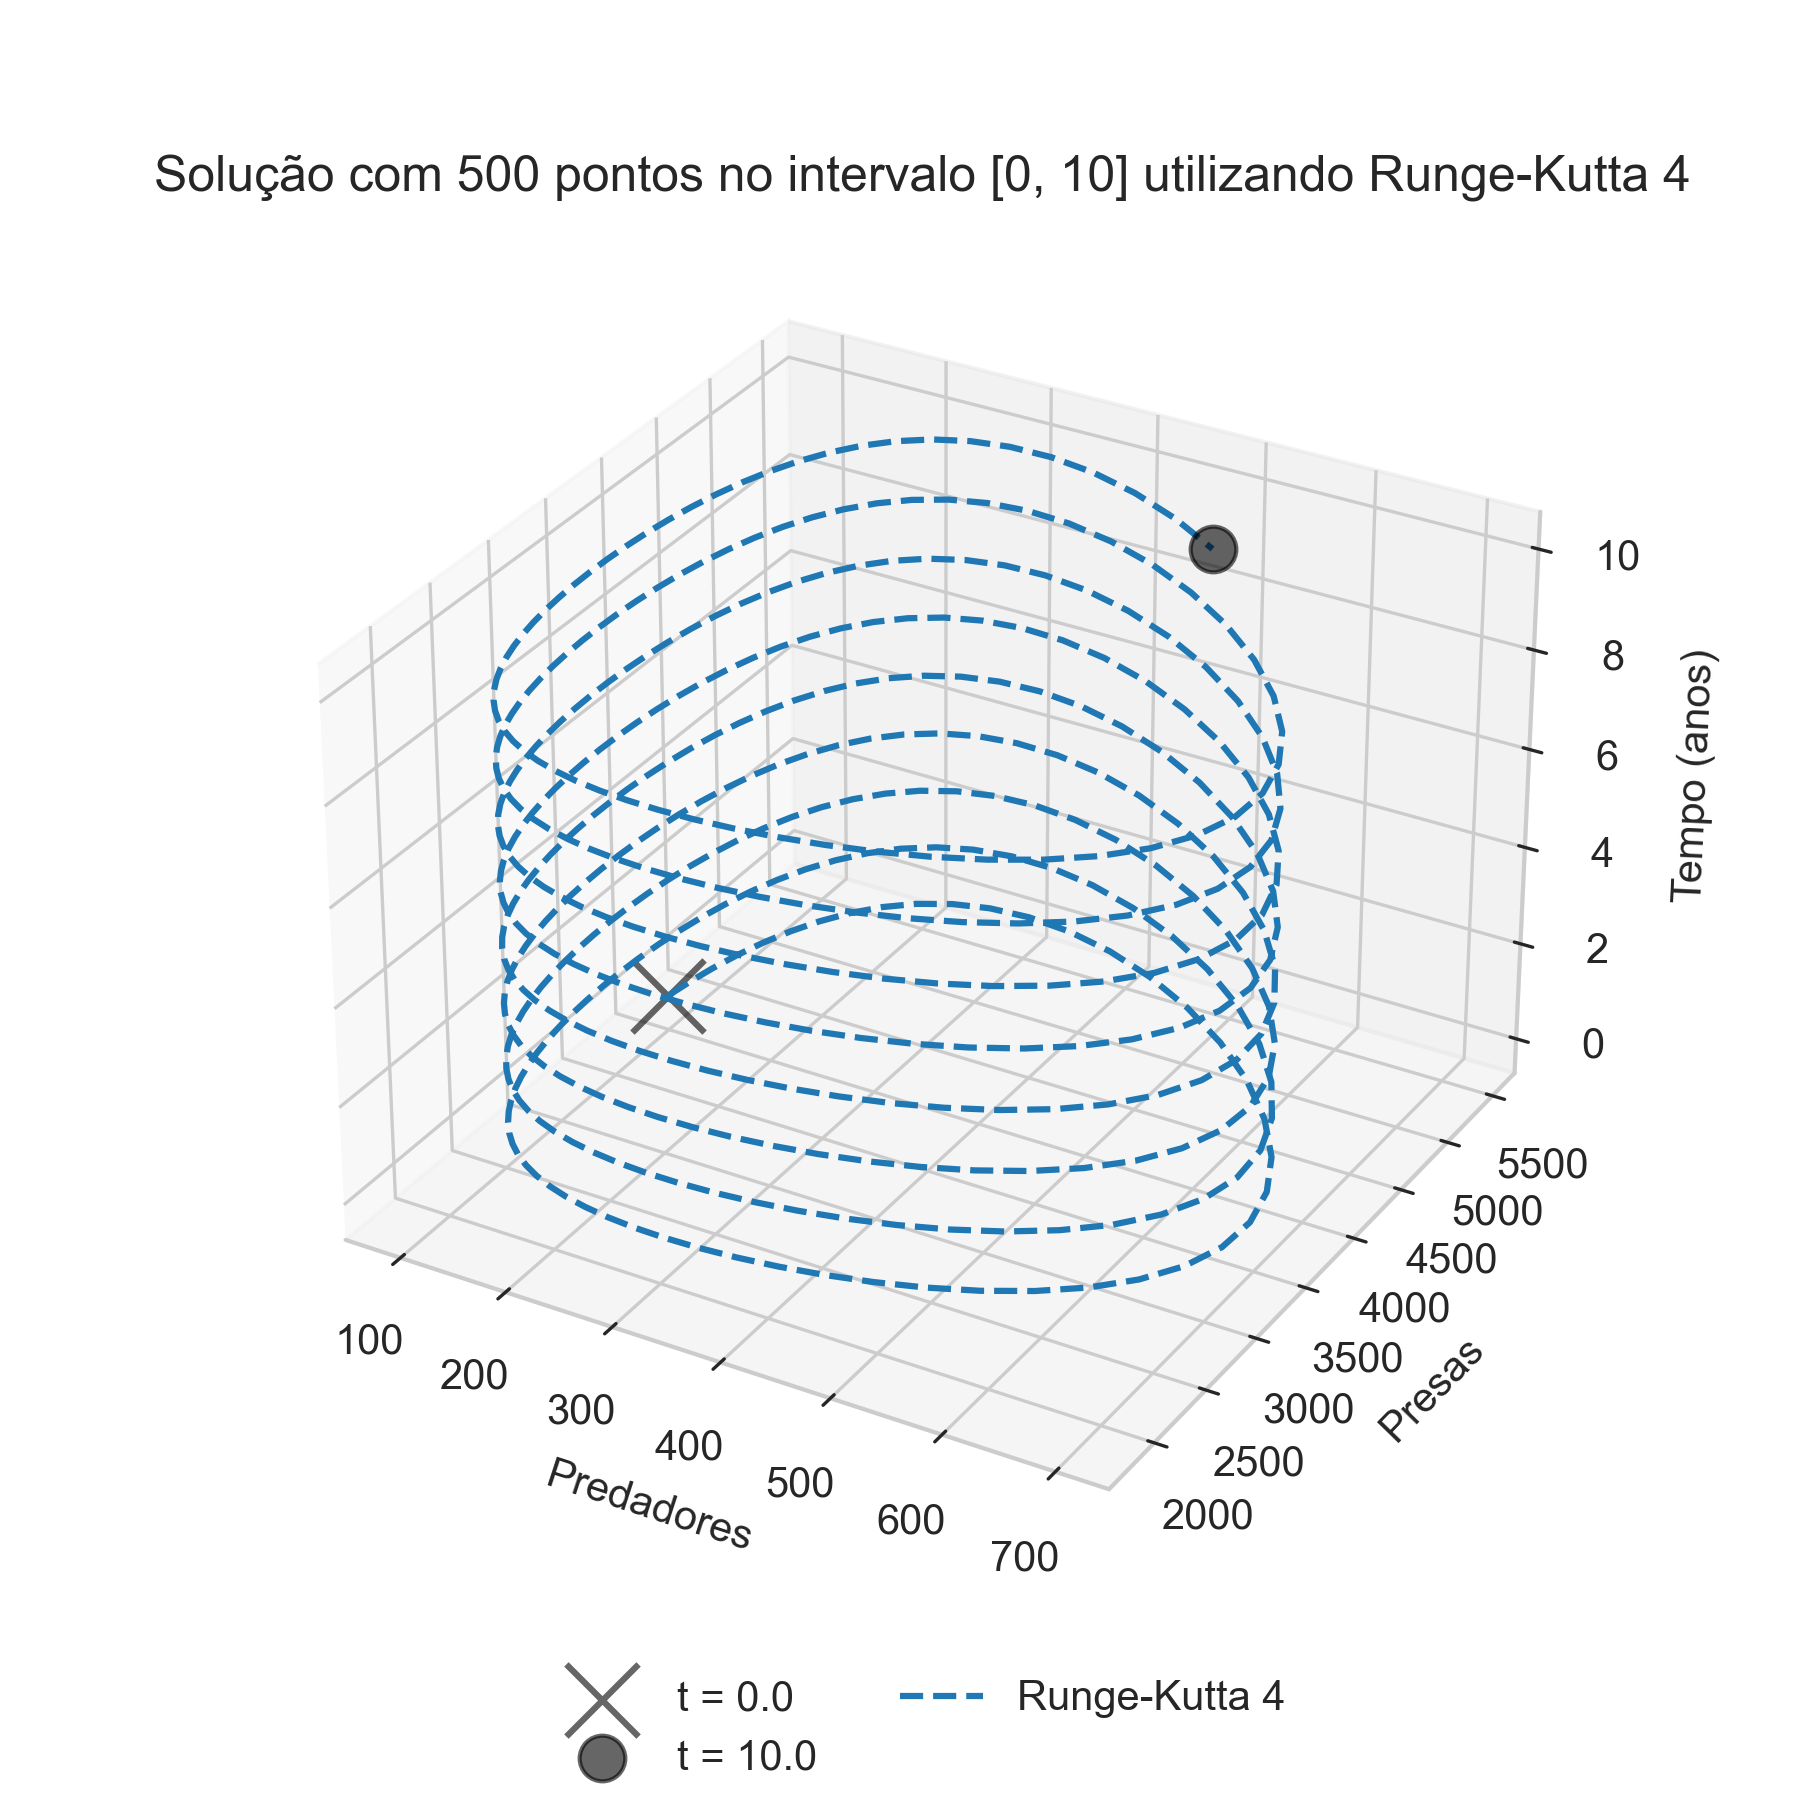
\includegraphics[height=12cm, width=12cm]{predator-prey/predator_prey-300dpi-Runge-Kutta_4-500 points.png}}
	}
	\caption{Método de Runge-Kutta de 4ª ordem - (a) Evolução de ambas populações temporalmente; (b) Número de indivíduos vivos simultaneamente em diferentes instantes de tempo; (c) Representação tridimensional da evolução do problema.}
    \label{img:rk4_plots}
\end{figure}

Constata-se que ambas soluções simulam de forma semelhante a relação de predação, onde a população de predadores cresce quando há muitas presas para se alimentar, assim como a população de presas cresce vertiginosamente quando há poucos predadores e vice-versa.

Na Figura \ref{img:explicit_euler_plots}, é possível observar que o método de Euler Implícito reduz a amplitude dos ciclos das populações ao longo do tempo, resultando em um comportamento espiral. A partir do início do intervalo, cada ano manteve o comportamento da curva, mas reduziu a variação da população. Embora novos indivíduos surjam e outros faleçam, a quantidade de indivíduos vivos simultaneamente tende a um valor constante.

Ao estudar a solução pelo método explícito de quarta ordem, observa-se que na Figura \ref{img:rk4_plots}, forma-se um gráfico periódico, em que cada ano reproduz o anterior identicamente.

Para verificar se os resultados convergem para a solução apropriada do problema, é utilizada a mesma técnica de refinamento de malha aplicada nos problemas (\ref{problem-1}) e (\ref{problem-2}). Essa técnica utiliza uma malha grossa, intermediária e fina para obter resultados cada vez mais precisos. Os resultados são ilustrados na Figura \ref{img:comparison_plots}.

\begin{figure}[H]
	\centering
	\mbox{
		\subfigure[]{
			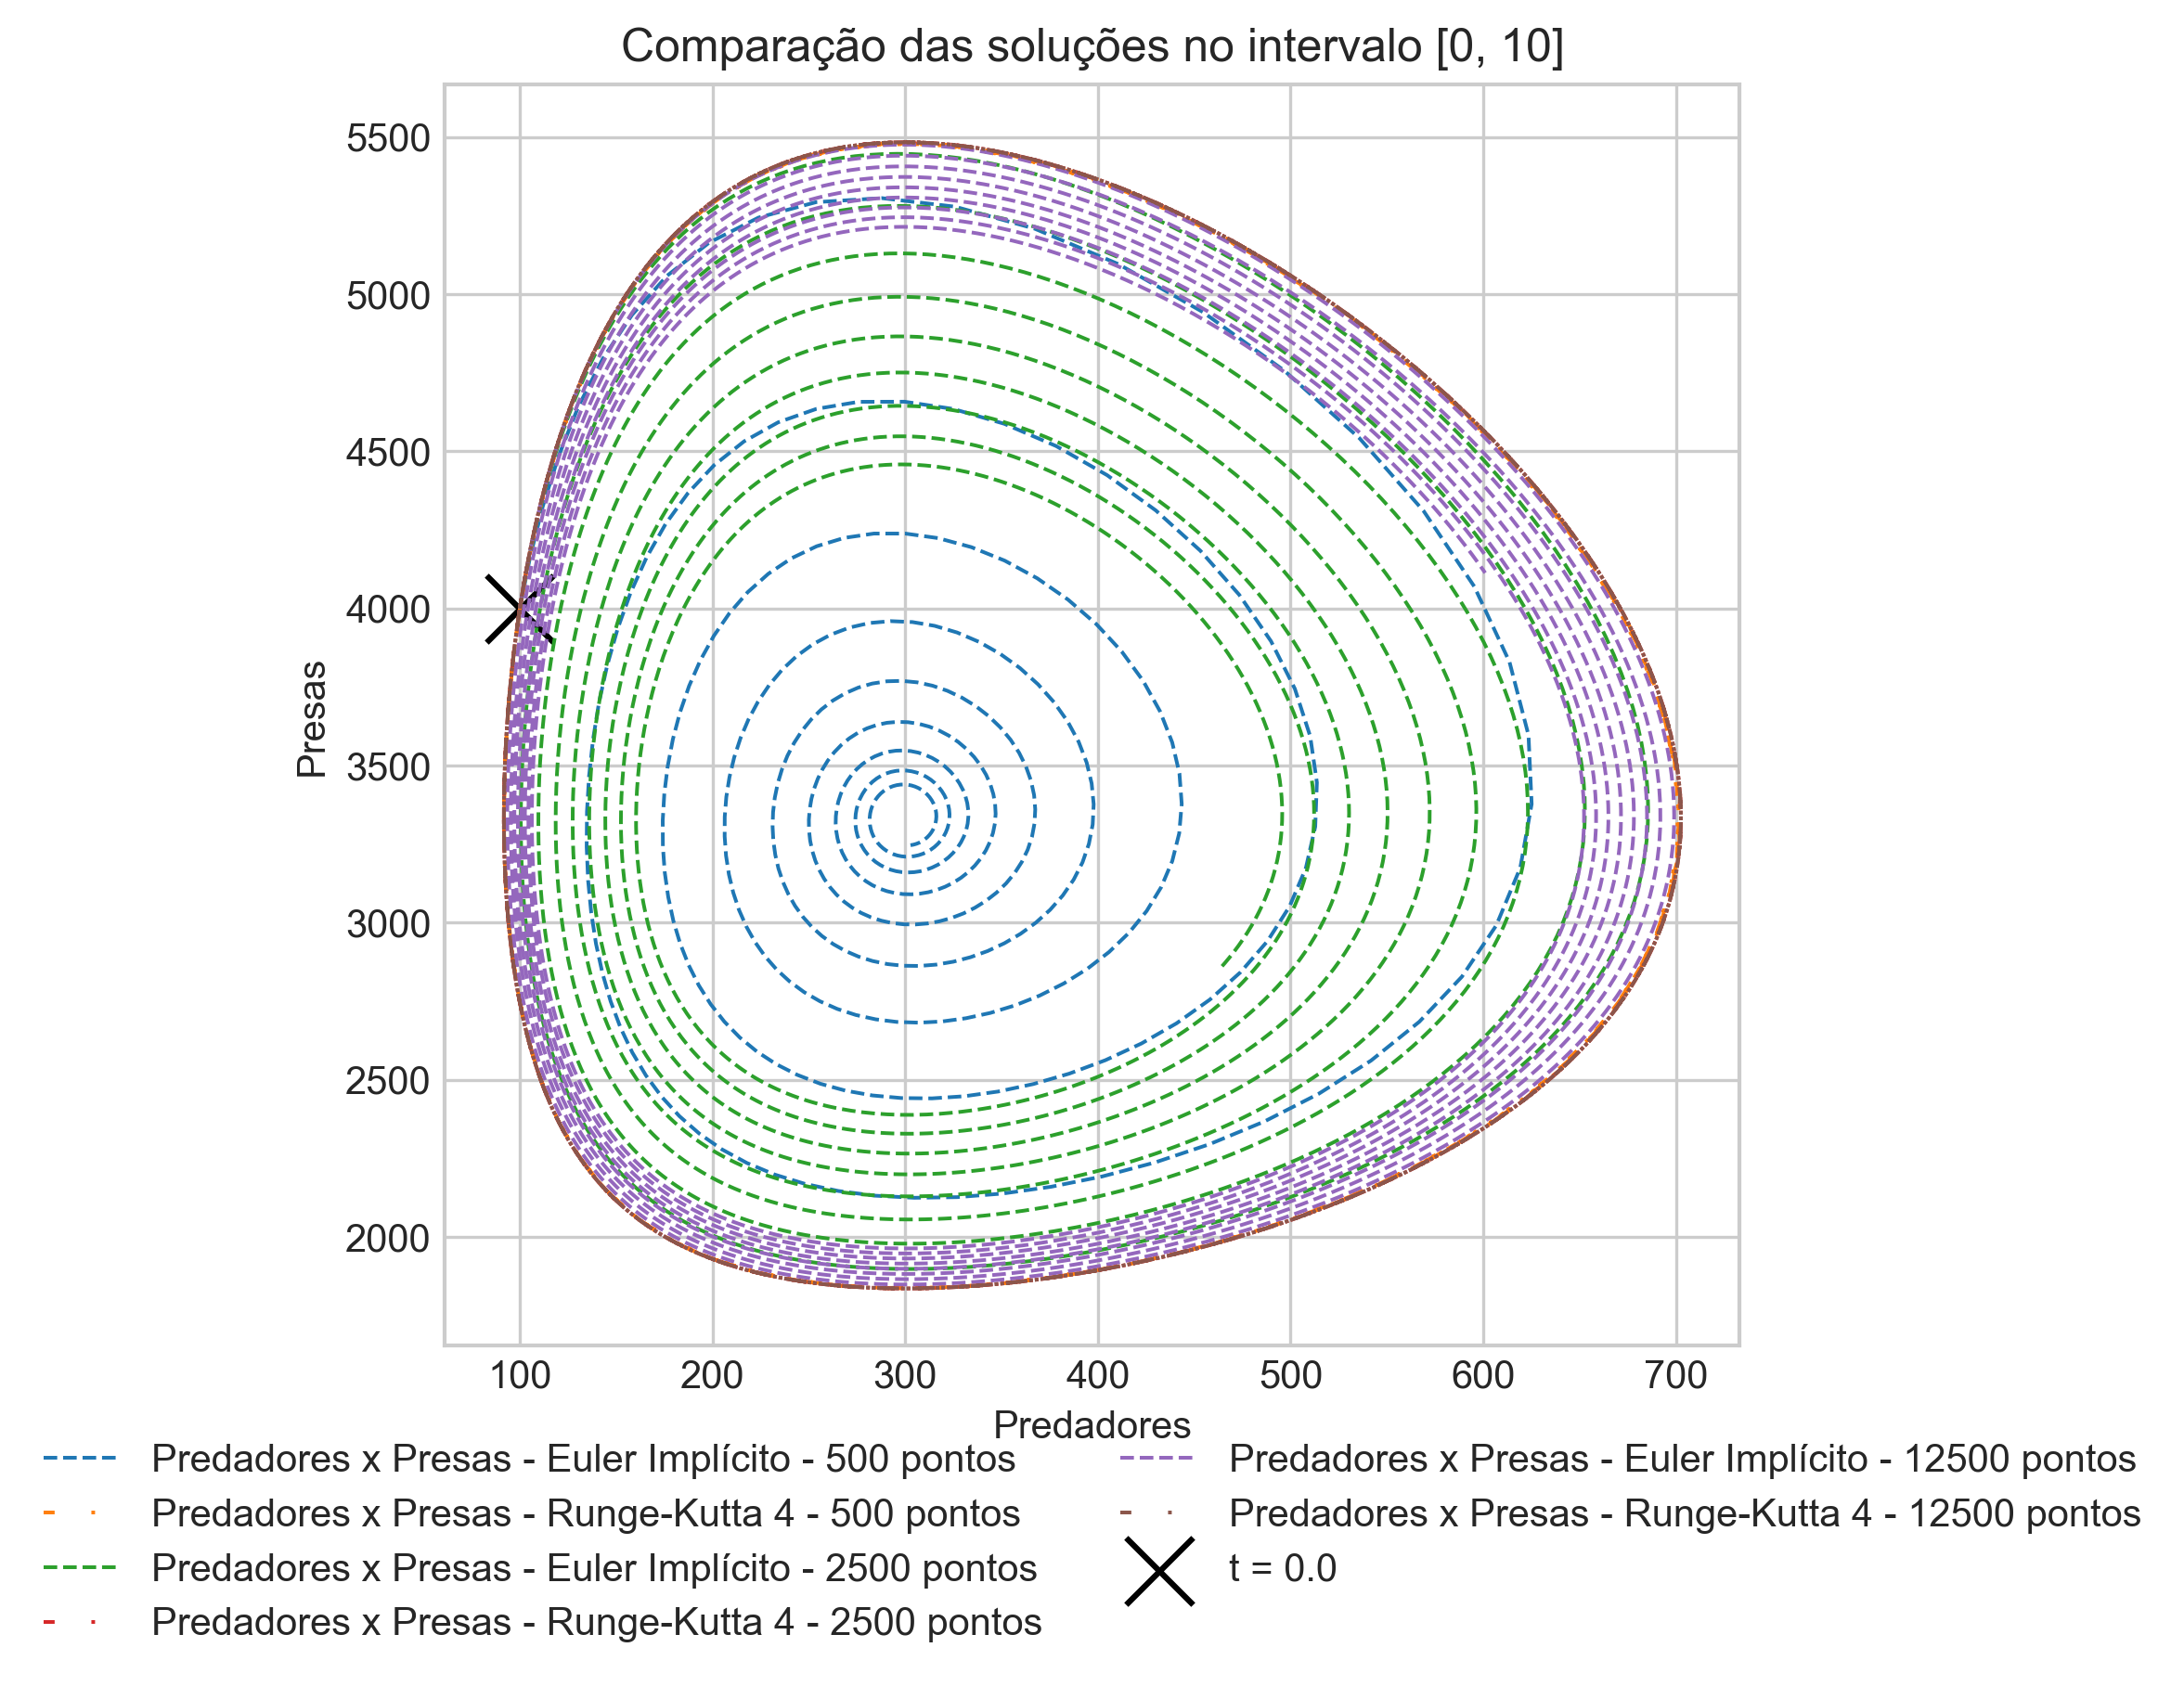
\includegraphics[height=10cm]{predator-prey/pp-comparison-2d.png}}
	}
   \mbox{
		\subfigure[]{
			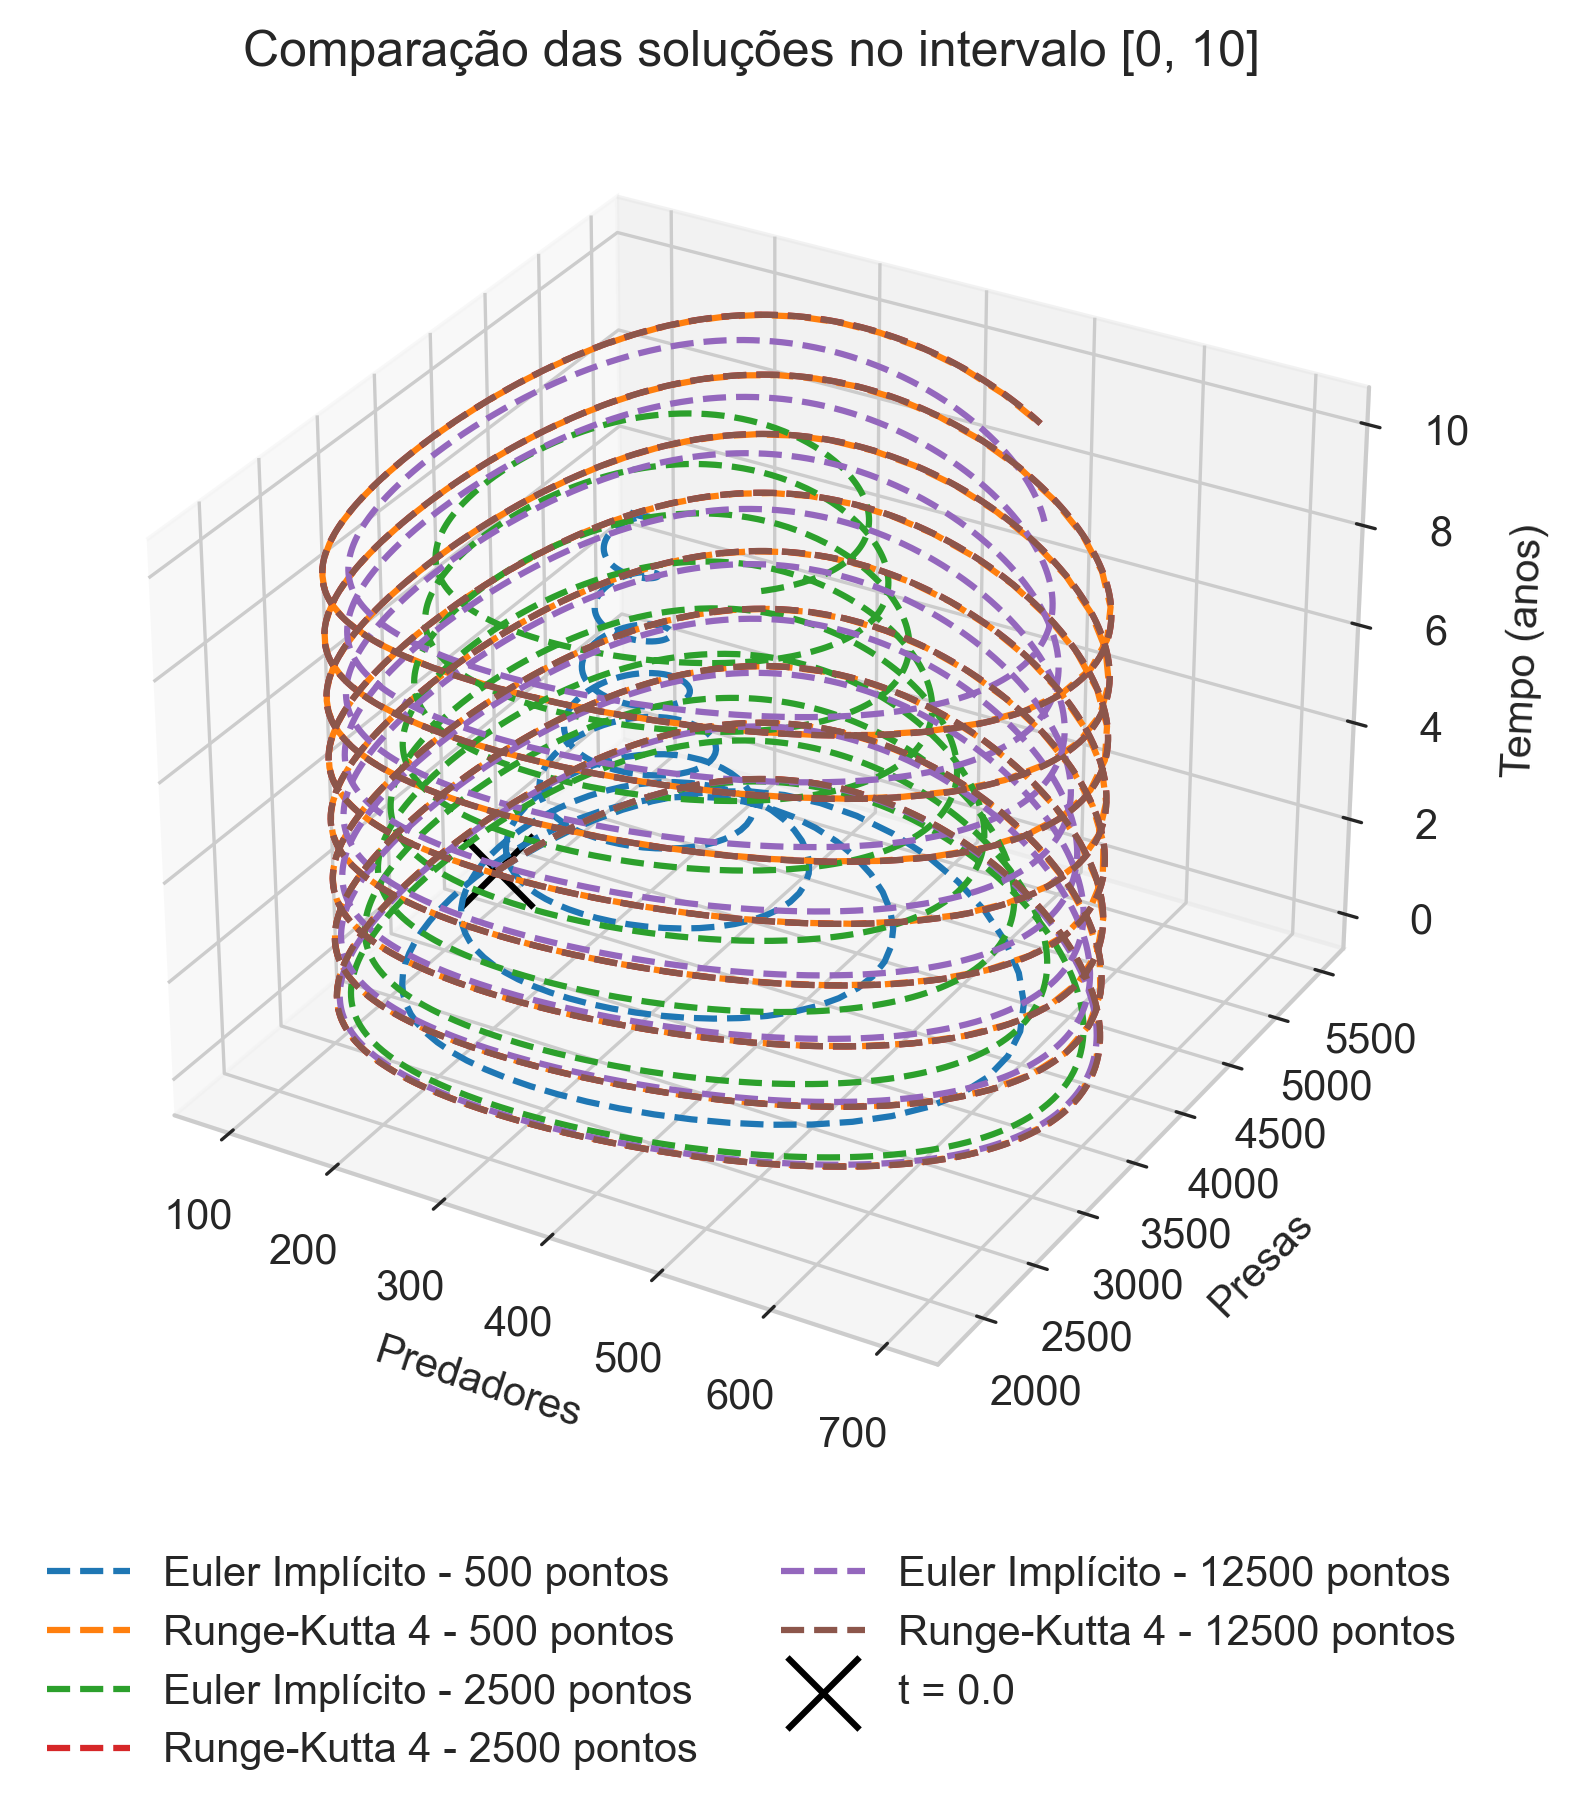
\includegraphics[height=10cm]{predator-prey/pp-comparison.png}}
   }
	\caption{(a) Representação bidimensional das soluções obtidas para distintas malhas; (b) Representação temporal das soluções obtidas}
    \label{img:comparison_plots}
\end{figure}

A Figura \ref{img:comparison_plots} mostra que o método de quarta ordem converge para a mesma solução, independentemente do refinamento da malha, evidenciando sua estabilidade e precisão numérica. Por outro lado, o método implícito apresentou maior sensibilidade ao refinamento da malha, tendo a solução se aproximado daquela obtida pelo método de Runge-Kutta. Apesar disso, o comportamento espiral ainda persiste no método implícito.

\begin{figure}[H]
	\centering
    \mbox{
        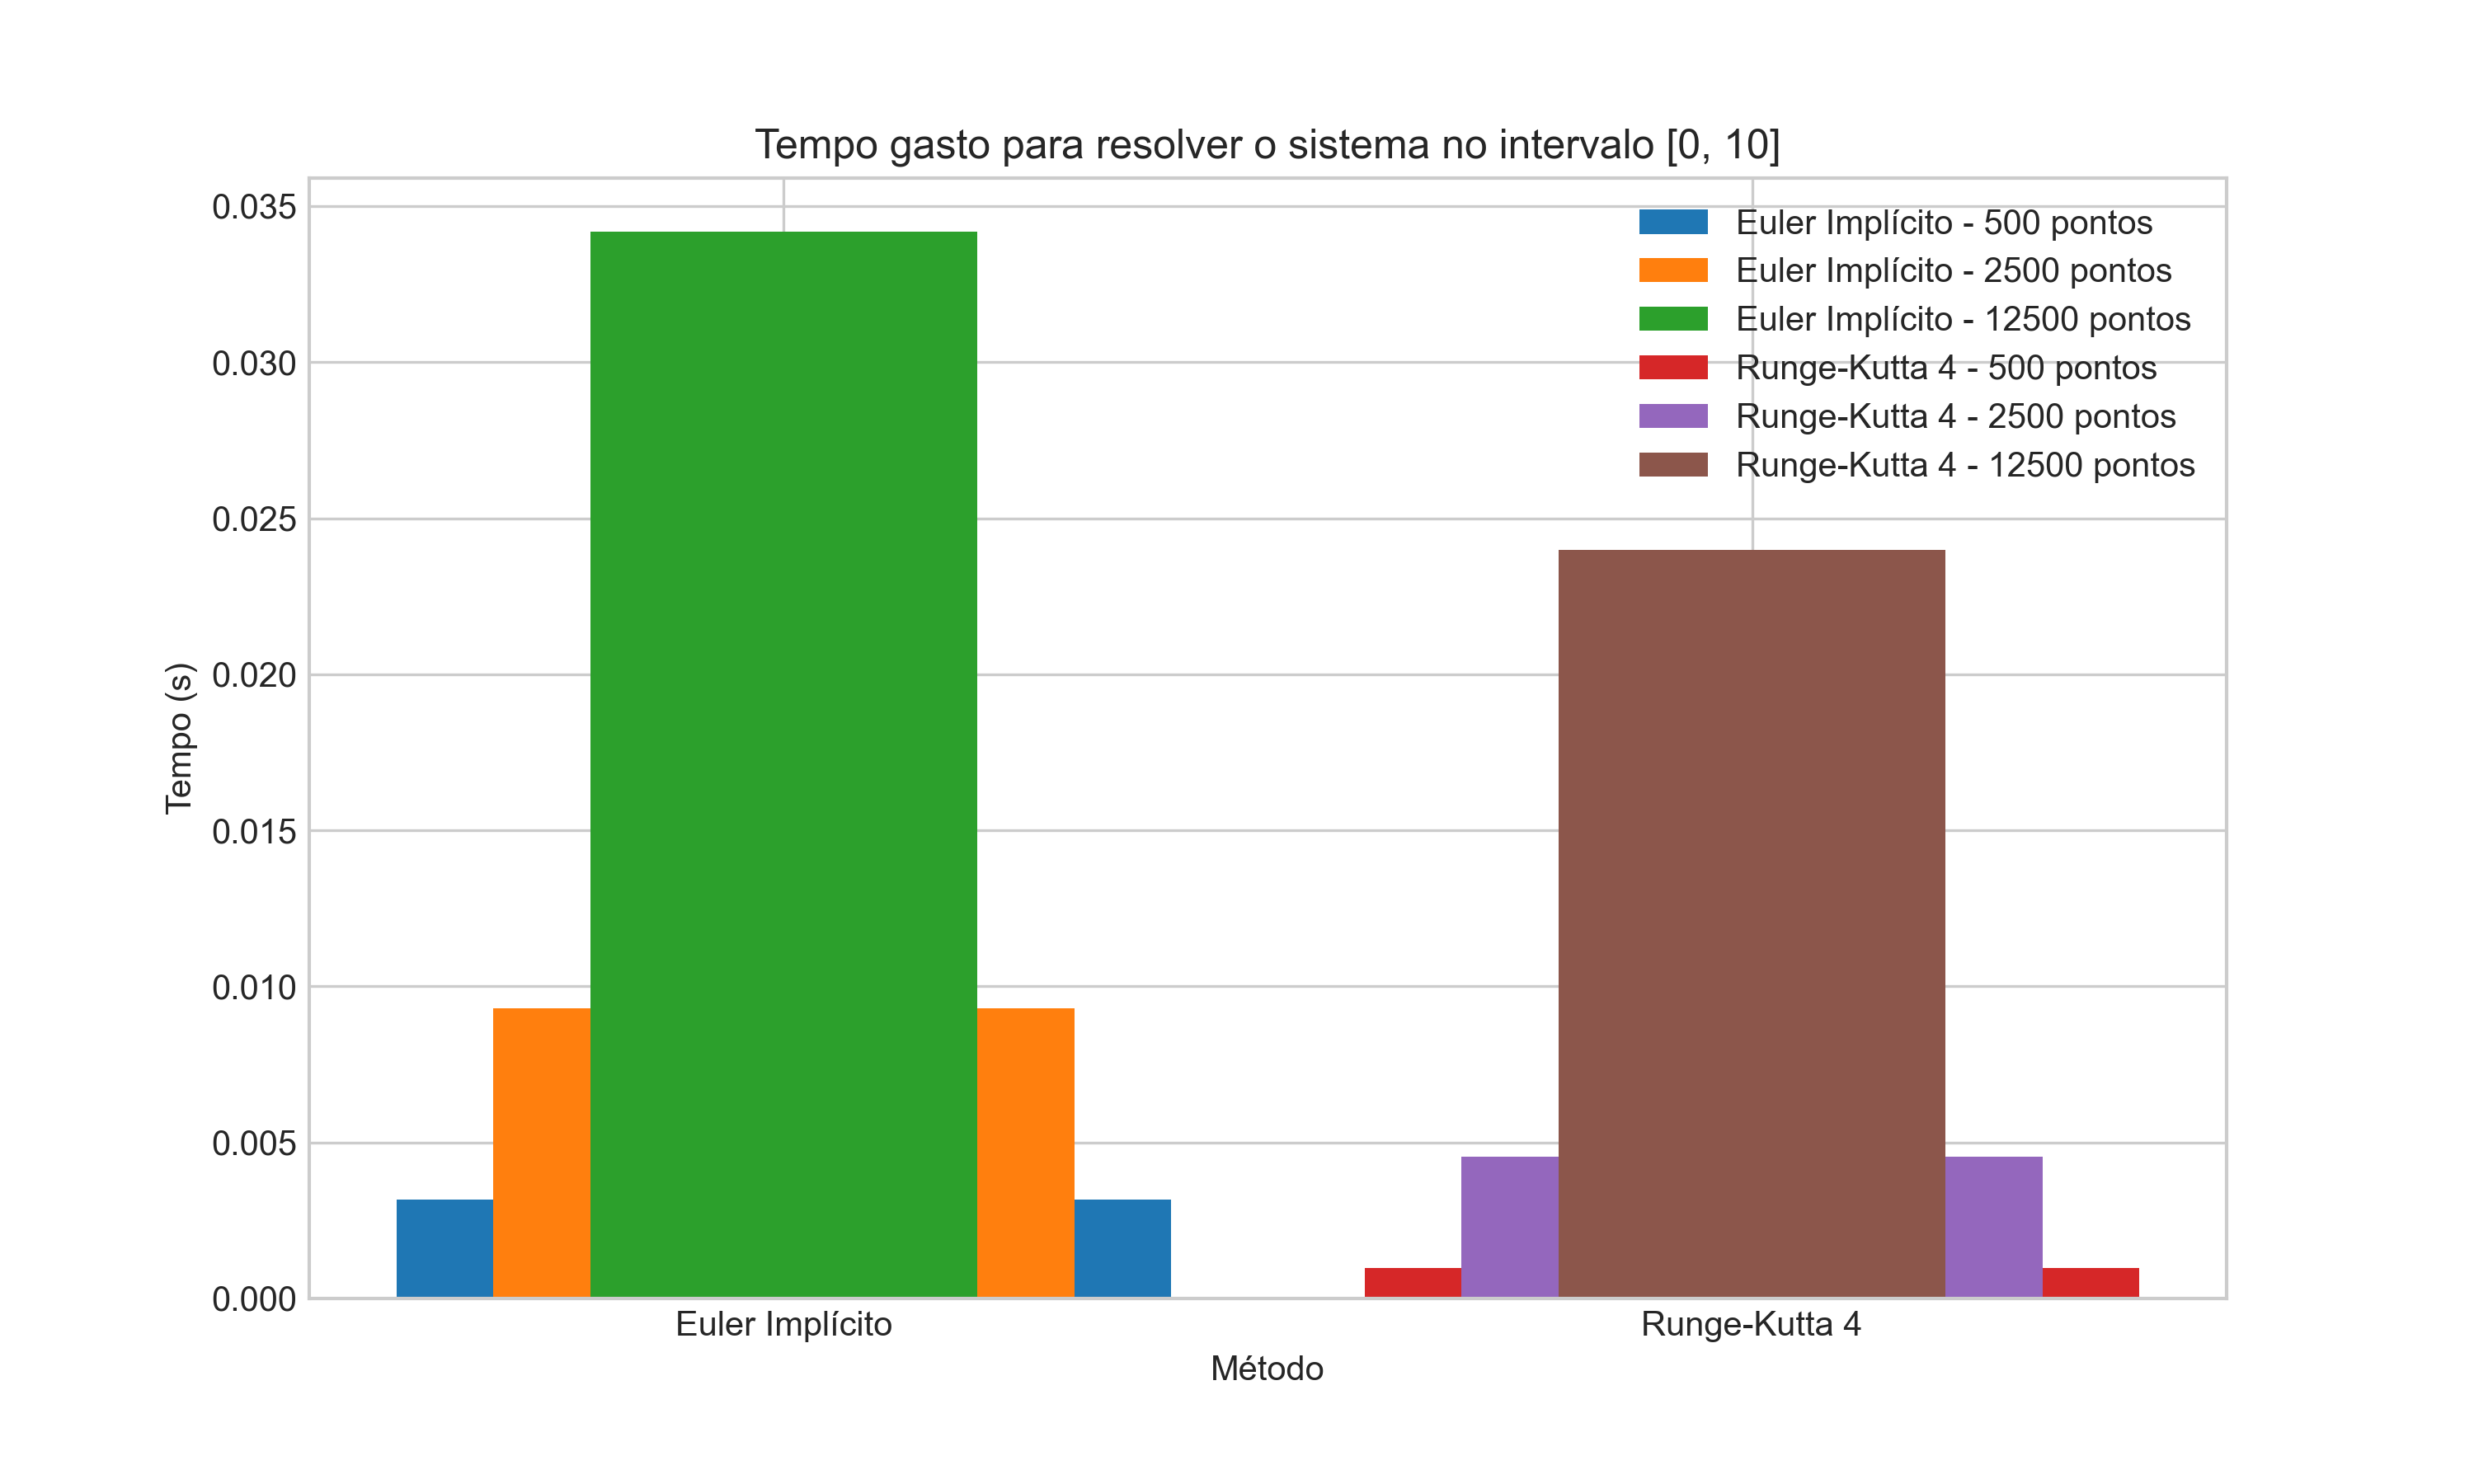
\includegraphics[width=14cm]{predator-prey/predator_prey-300dpi-time-comparison.png}
    }
	\caption{Tempo gasto para resolver o sistema.}
    \label{img:pp-times}
\end{figure}

Considerando a Figura \ref{img:comparison_plots}, é possível observar que ambos os métodos estão convergindo para a solução, porém, em velocidades distintas. É importante destacar que a escolha de um método dependerá da precisão e eficiência computacional desejadas. Nesse sentido, o método de quarta ordem pode ser considerado o mais adequado para este problema, uma vez que obteve uma solução melhor com uma quantidade de pontos bastante inferior ao método de primeira ordem, economizando tempo de processamento computacional, conforme apresentado na Figura \ref{img:pp-times}.